\setcounter{section}{7}
\addsec{Versuch 7}


\subsection{Verhalten einer Zenerdiode}
\begin{figure}[H]
	\centering
	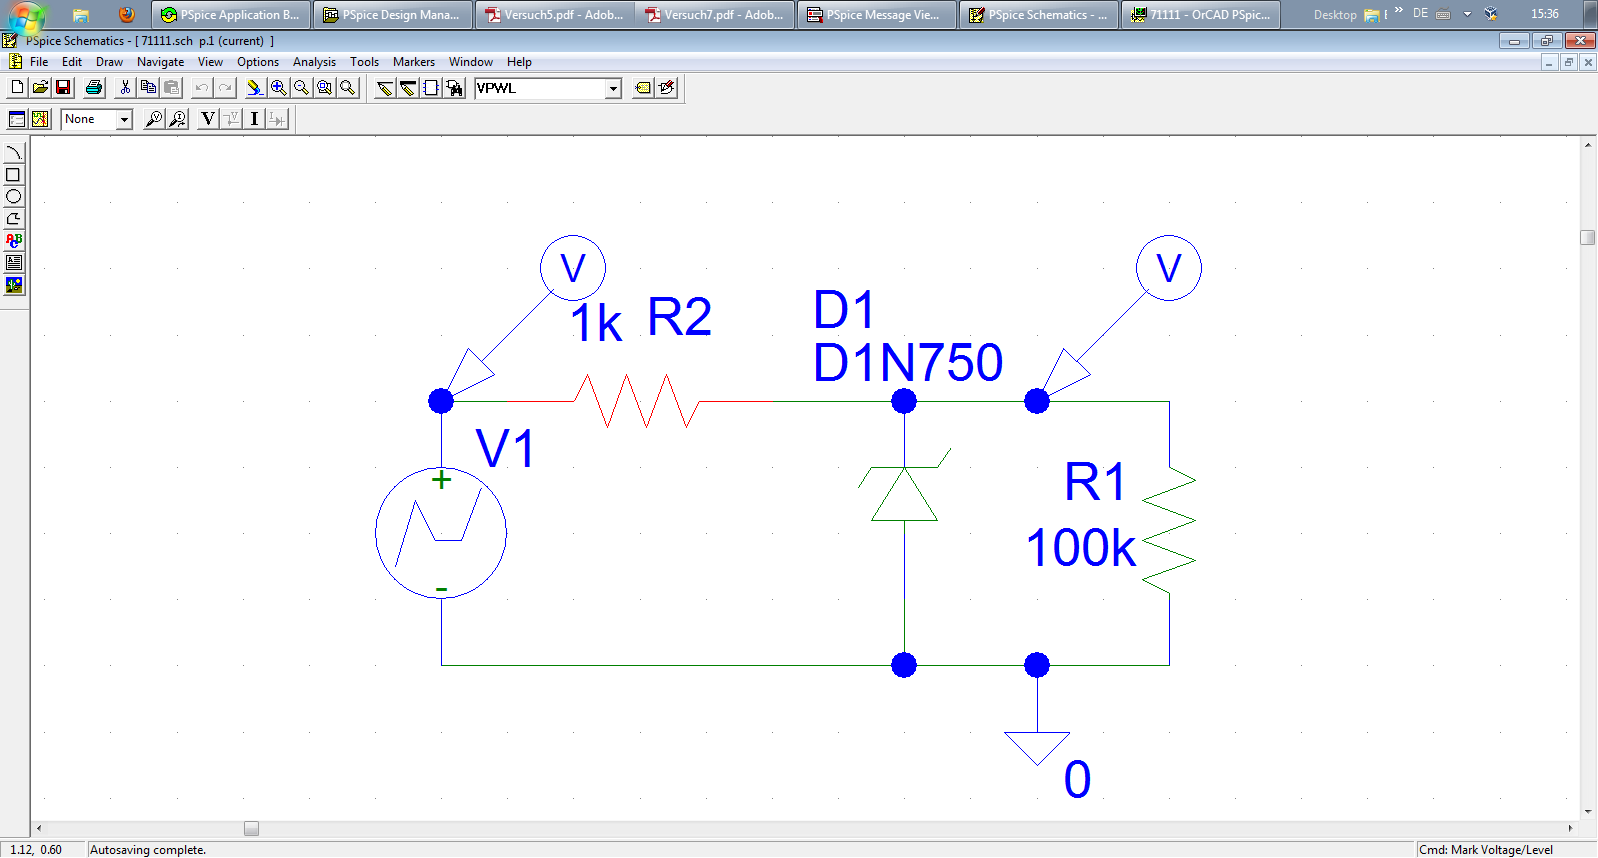
\includegraphics[width=\linewidth]{versuch7/spice/s7111.png}
	\caption{Schaltplan, wie im Skript vorgegeben}
\end{figure}
\begin{figure}[H]
	\centering
	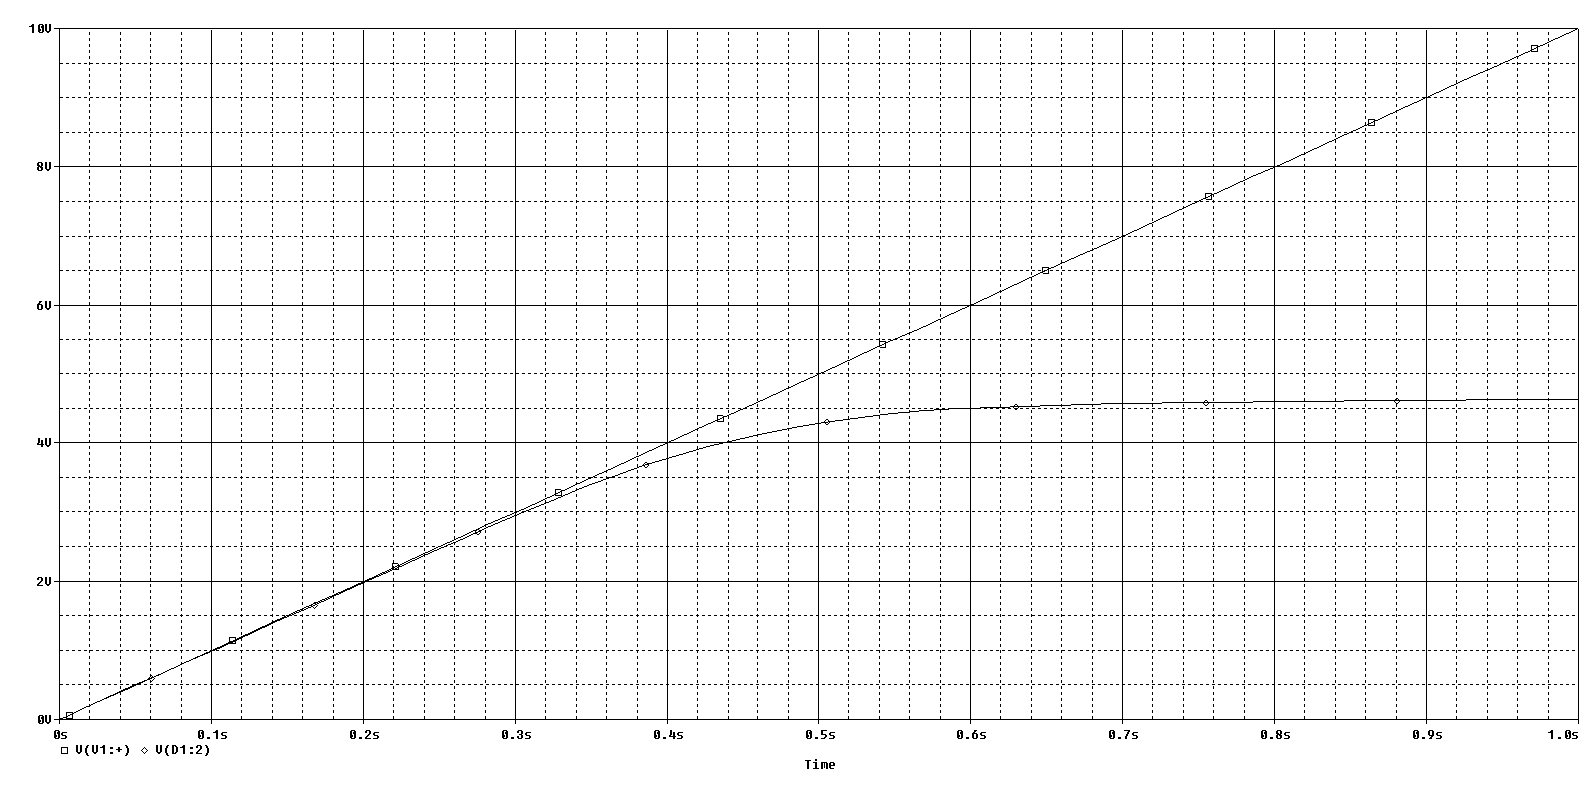
\includegraphics[width=\linewidth]{versuch7/spice/7111.png}
	\caption{Simulationsergebnis}
\end{figure}
Die Diode besitzt eine Durchbruchspannung von 4.5V. Bei 7V Eingangsspannung werden 4.5682V gemesseen, bei 10V misst man 4.6267V. Damit folgt für die Güte der Stabilisierung:
\[ Q=\frac{\Delta U_{EIN}}{\Delta_{AUS}} = \frac{10V-7V}{4.6267V-4.5682V}=51.282 \]
Wenn man die Zenerdiode ohne Vorwiderstand an einer Spannungsquelle betreibt, kann sie schlichtweg nicht funktionieren.


\subsection{Konstantstromquelle mit FET}
\begin{figure}[H]
	\centering
	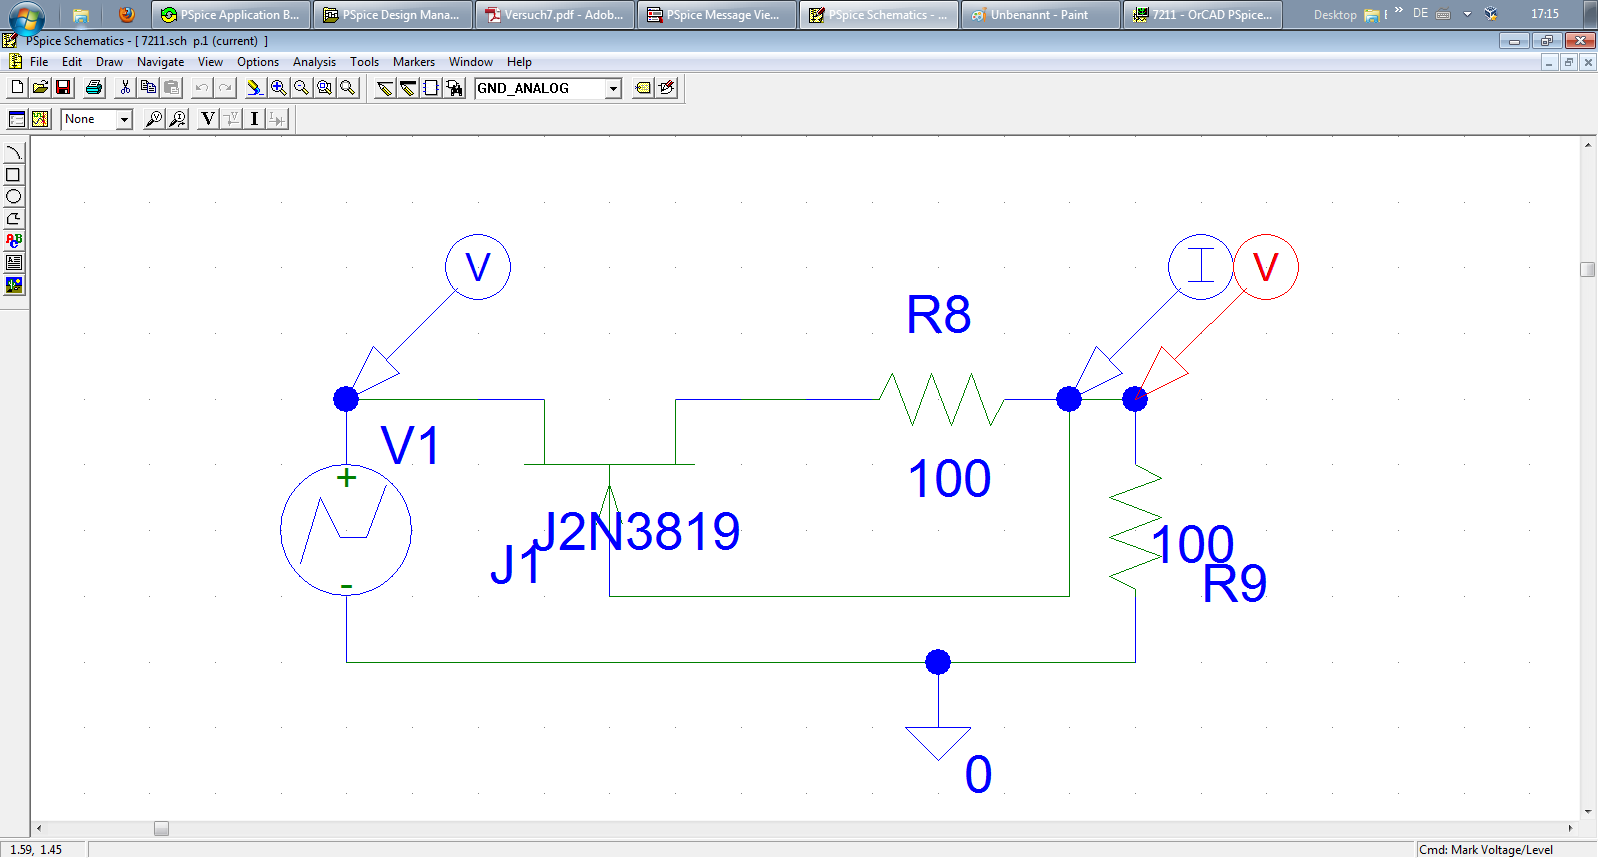
\includegraphics[width=\linewidth]{versuch7/spice/s7211.png}
	\caption{Schaltplan, wie im Skript vorgegeben}
\end{figure}
\begin{figure}[H]
	\centering
	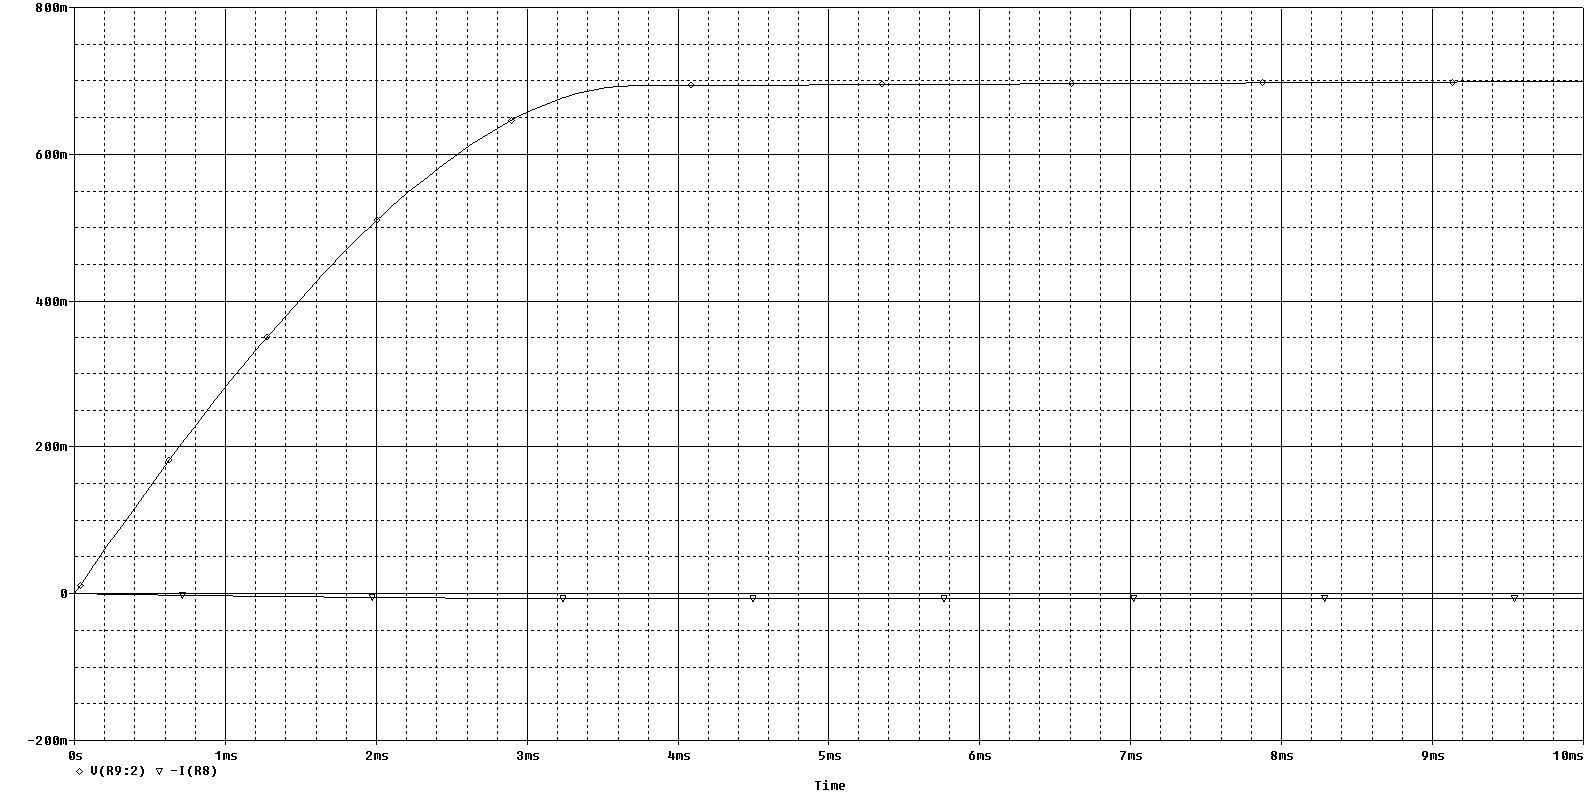
\includegraphics[width=\linewidth]{versuch7/spice/7212.png}
	\caption{Simulationsergebnis}
\end{figure}
Bei 8ms beträgt der Strom durch den Transistor 6.9739mA.\\
Als nächstes wurder der Lastwiderstand auf 500k\Ohm erhöht. Nun beträgt der Strom nach 8ms 6.9473mA.\\
Ja, ich könnte mir vorstellen, wie man so ein Messgerät zur Widerstandsmessung bauen könnte\footnote{Es gilt $ U=R*I $, also $ R=\frac{U}{I} $. Wenn man also mit der Stromquelle den Strom vorgibt, besteht ein linearer Zusammenhang zwischen der Spannung und dem Widerstand. Man muss also nur die Zahl der Spannung mit dem Strom skalieren und die Einheit als Ohm ausgeben.}.


\subsection{Entwurf einer einfachen Referenzspannungsquelle}
Wie wir in Versuch 1 gesehen haben, hängt der Spannungsabfall an der Zenerdiode für große Ströme näherungsqweise linear vom Strom ab. Die Zenerdiode bildet mit dem Innenwiderstand einen Spannungsteiler der mit steigender Spannung mit steigendem Strom durchflossen wird. Daher wird die Spannungsstabilisierung deutlich verbessert, wenn der Anstieg dieses Stroms gebremst wird. Genau dies geschiegt, wenn man den Widerstand durch eine Konstantstromquelle ersetzt.
\subsubsection*{Simulation}
\begin{figure}[H]
	\centering
	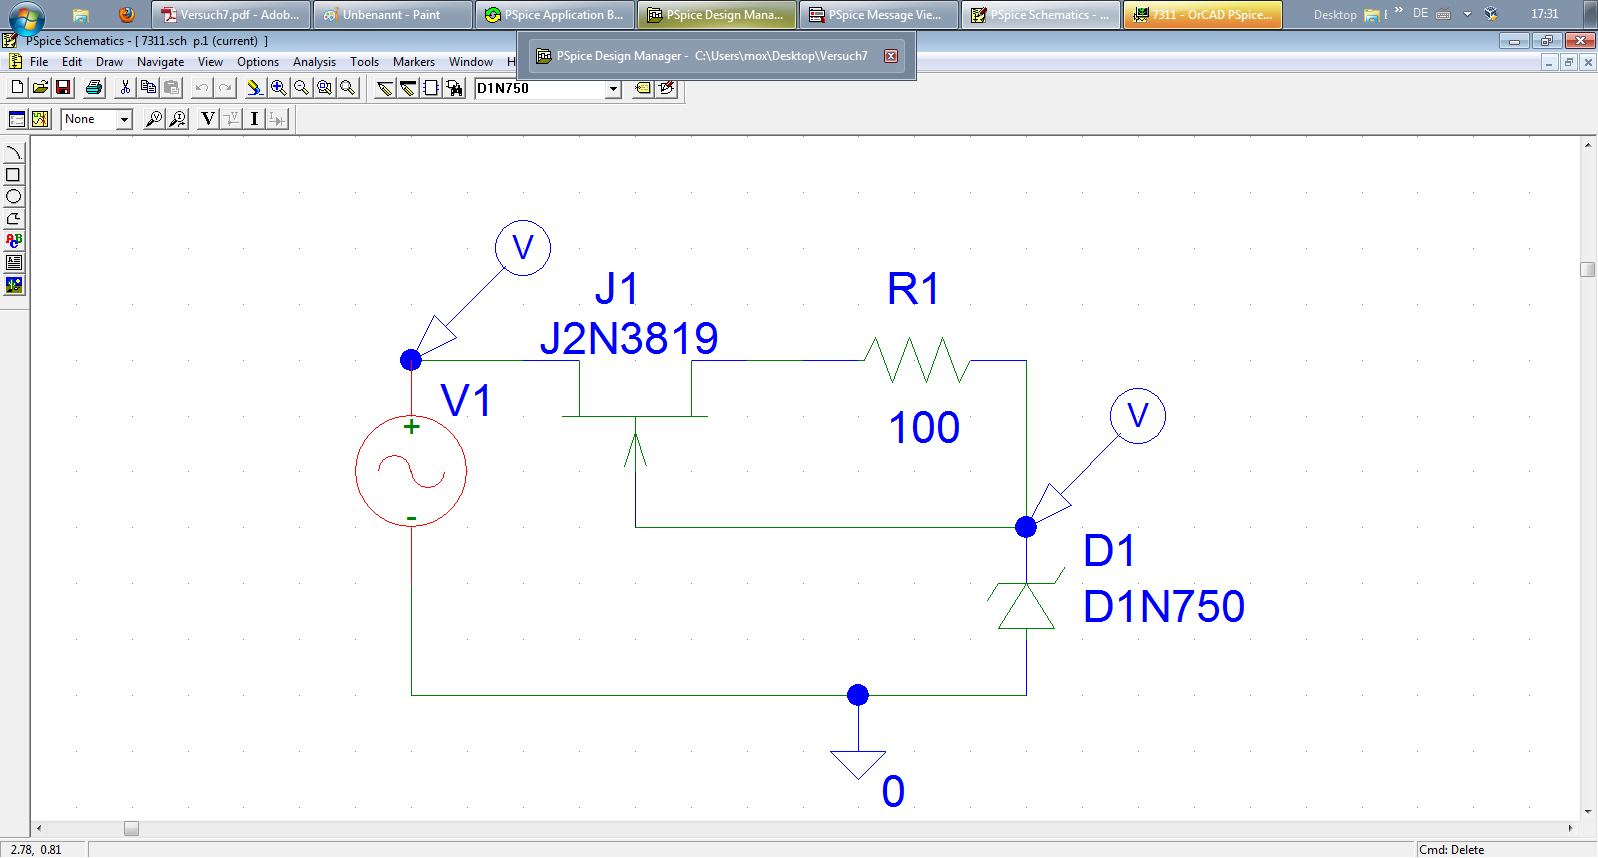
\includegraphics[width=\linewidth]{versuch7/spice/s7311.png}
	\caption{Schaltplan, wie im Skript vorgegeben}
\end{figure}
\begin{figure}[H]
	\centering
	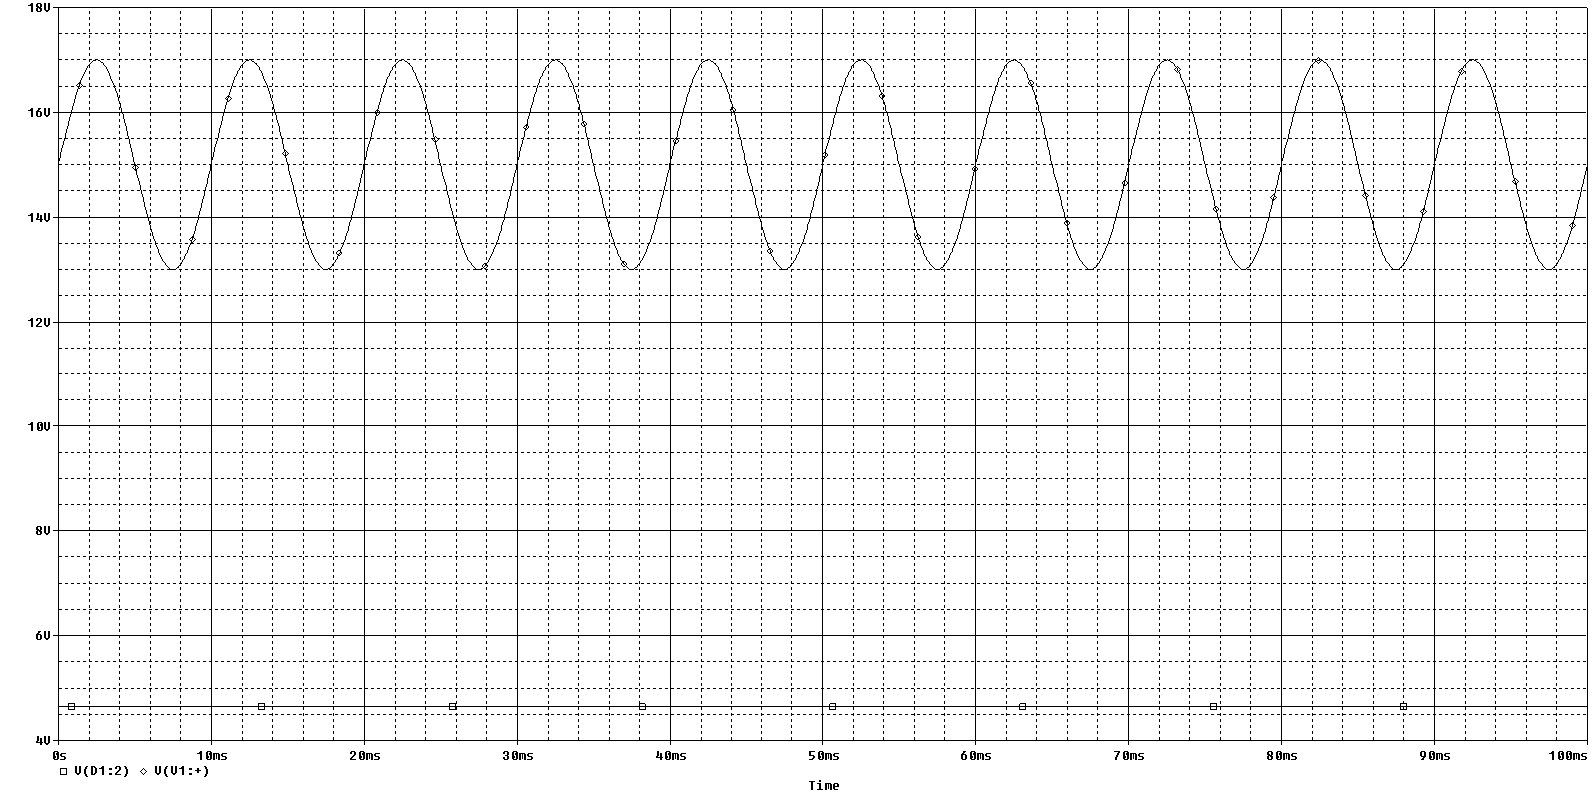
\includegraphics[width=\linewidth]{versuch7/spice/7311.png}
	\caption{Simulationsergebnis}
\end{figure}
Die Variation der Zenerspannung beträgt: 312.805µV
\subsubsection*{Messung}
Die simulierte Schaltung wurde real aufgebaut und getestet.\\
Bei 10V Eingangsspannung betrug die Ausgangsspannung 4.7472V, bei 15V wurden 4.7492V gemessen. Somit ergibt sich ein Stabilisierungsfaktor von:
\[ Q=\frac{\Delta U_{EIN}}{\Delta_{AUS}} = \frac{15V-10V}{4.7492V-4.7472V}=2500.0 \]
Somit wird offenkundig, wie viel besser diese Spannungsstabilisierung ist.

\subsection{Linearregler I}
Um den Widerstand $ R_4 $ zu berechnen geht man wie folgt vor:
\begin{itemize}
	\item Zuerst bestimmt man die Spannung $ V_+ $. Sie beträgt, wie im vorigen Versuch bestimm, ca. 4.75V.
	\item Dann bestimmt man die Spannung an $ V_- $. Für sie gilt: $ V_- = U_{out} * \frac{R_3}{R_3+R_4} $

	\item Nach dem einfachen Transistormodel wird der Opamp seine Ausgangsspannung so treiben, dass $ V_- $ gegen $ V_+ $ geht, wir nehmen also $ V_+ = V_- $ an.\\Ausserdem soll $ V_{out} = 10V \pm 1\% $ gelten.

	\item Somit gilt: $ 4.75V = V_{out} * \frac{4.7k\Ohm}{4.7\Ohm+R_4} \Rightarrow R_4 = \left( \frac{V_{out}}{4.75V} *4.7k\Ohm \right) -4.7k\Ohm$
\end{itemize}

Für $ R_4 $ gilt somit: \[ V_{out} \in \left[ 9.9V , 10.1V \right]  \leadsto R_4 \in \left[ 5095.8\Ohm,\; 5293.7\Ohm \right] \leadsto R_4 = 5194.7\Ohm \pm 1.9048 \% \]

\begin{figure}[H]
	\centering
	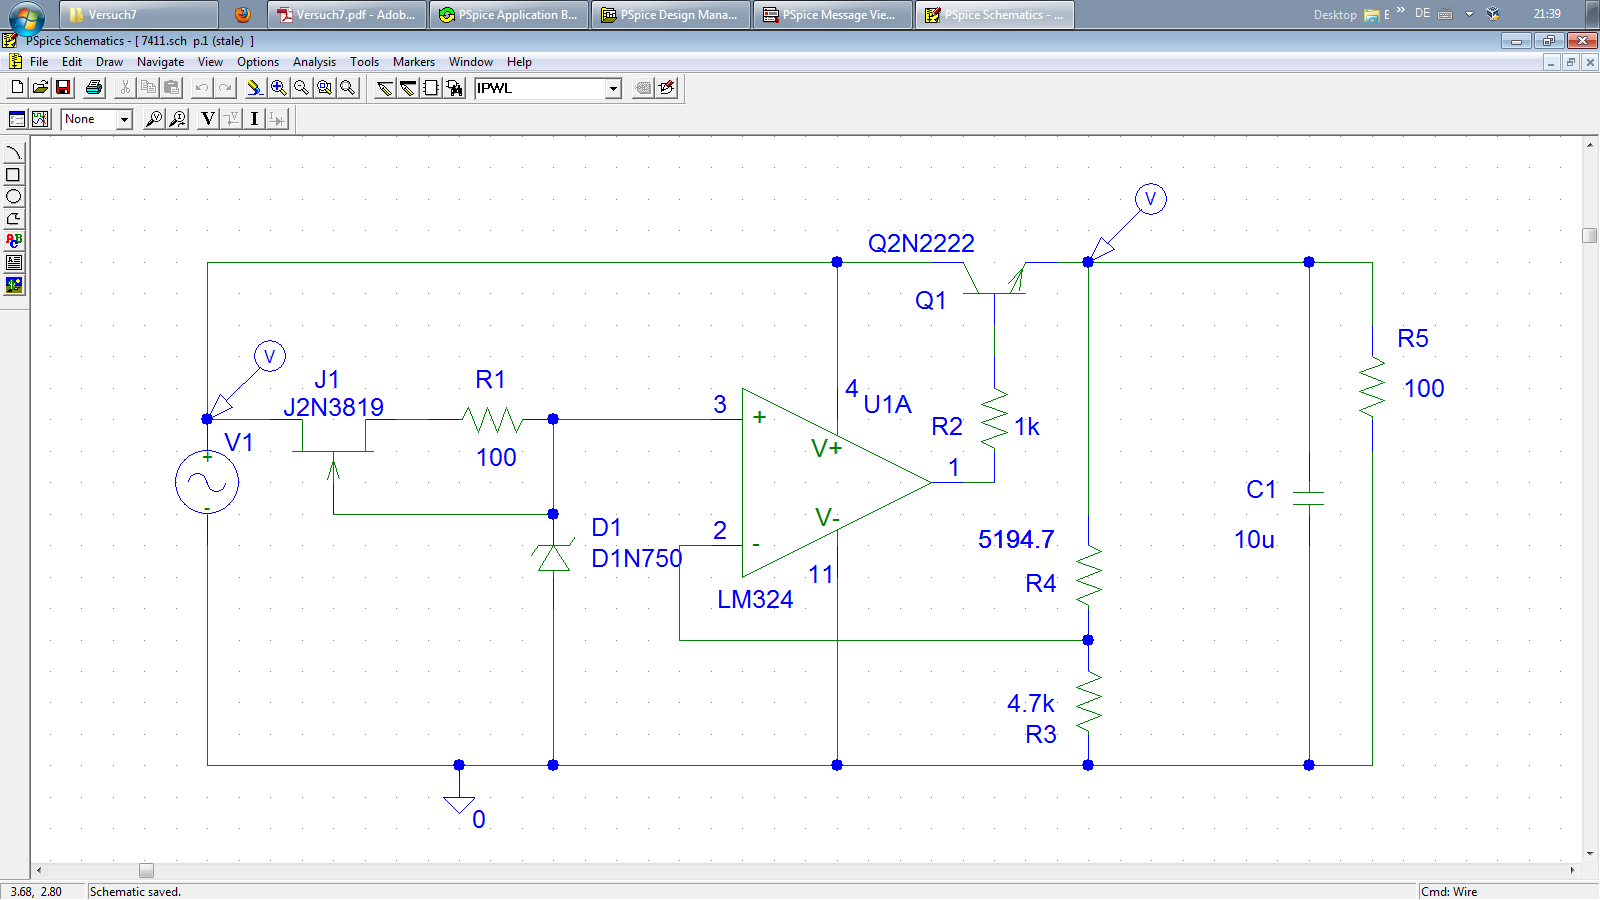
\includegraphics[width=\linewidth]{versuch7/spice/s7411.png}
	\caption{Schaltplan: Der Steuerspannungsteiler wurde deutlicher hervorgehoben}
\end{figure}
\begin{figure}[H]
	\centering
	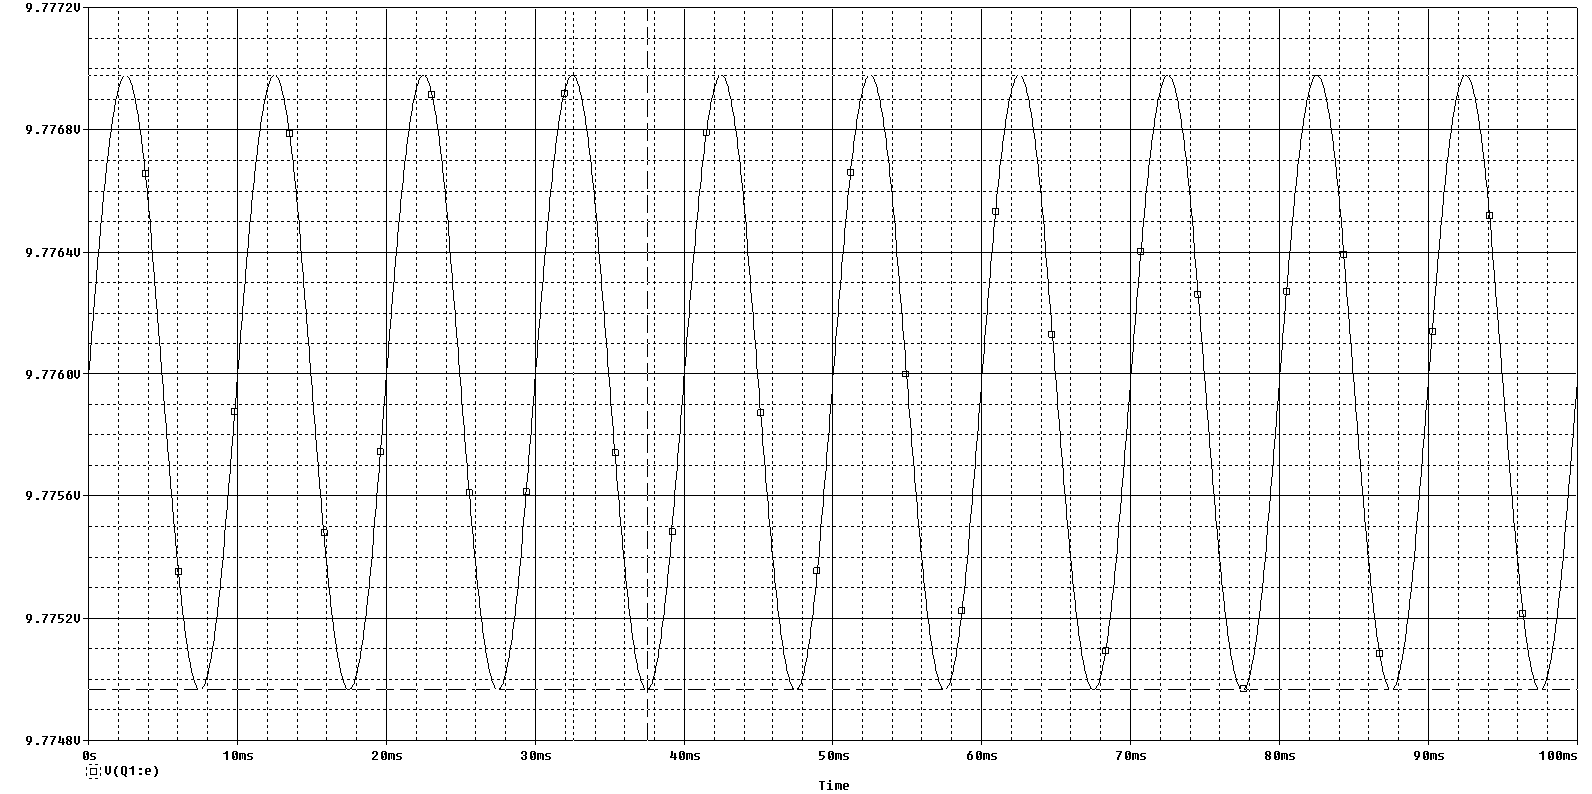
\includegraphics[width=\linewidth]{versuch7/spice/7411.png}
	\caption{Simulationsergebnis bei $ V_{Ampl} = 2V,\; V_{Offset} = 15V $}
\end{figure}
Die Welligkeit der Ausgangsspannung, $ U_{ss} $ wurde zu 2.0131mV bestimmt, für die Stabilisierung ergab sich:
\[ Q=\frac{\Delta U_{EIN}}{\Delta_{AUS}} = \frac{4V}{2.0131mV}=1987 \]
Die Güte der Stabilisierung ist etwas schlechter als bei der Referenzspannungsquelle, weil die Ausgangsspannung verdoppelt wurde. Setzte man $ R_4 $ gleich 0\Ohm, so würde die Spannung zu 4.75V stabilisiert und die Stabilisierung hätte eine Güte von 4186.9.

Wenn man den Ausgang mit 0.1\Ohm kurzschliest, misst man die folgenden Werte:
\begin{itemize}
	\item $ V_{cc} = 15V $
	\item $ V_{out} = 0.094687V $
	\item $ I_{out} = 0.946883A $
\end{itemize}
Somit ergibt sich am Transistor:
\begin{itemize}
	\item $ V_{drop} = V_{cc} - V_{out} = 14.905V $
	\item $ P = V_{drop} * I_{out} = 14.114W \Rightarrow $ 
\includegraphics[height=1.5\baselineskip]{versuch7/kaboom.png}\footnote{Quelle: \url{http://themoderatevoice.com/141180/talk-radio-bomb-98-advertisers-tell-\premiere-networks-to-avoid-shock-jocks}}
\end{itemize}
\subsection{Linearregler II}
\subsubsection*{Simulation}
\begin{figure}[H]
	\centering
	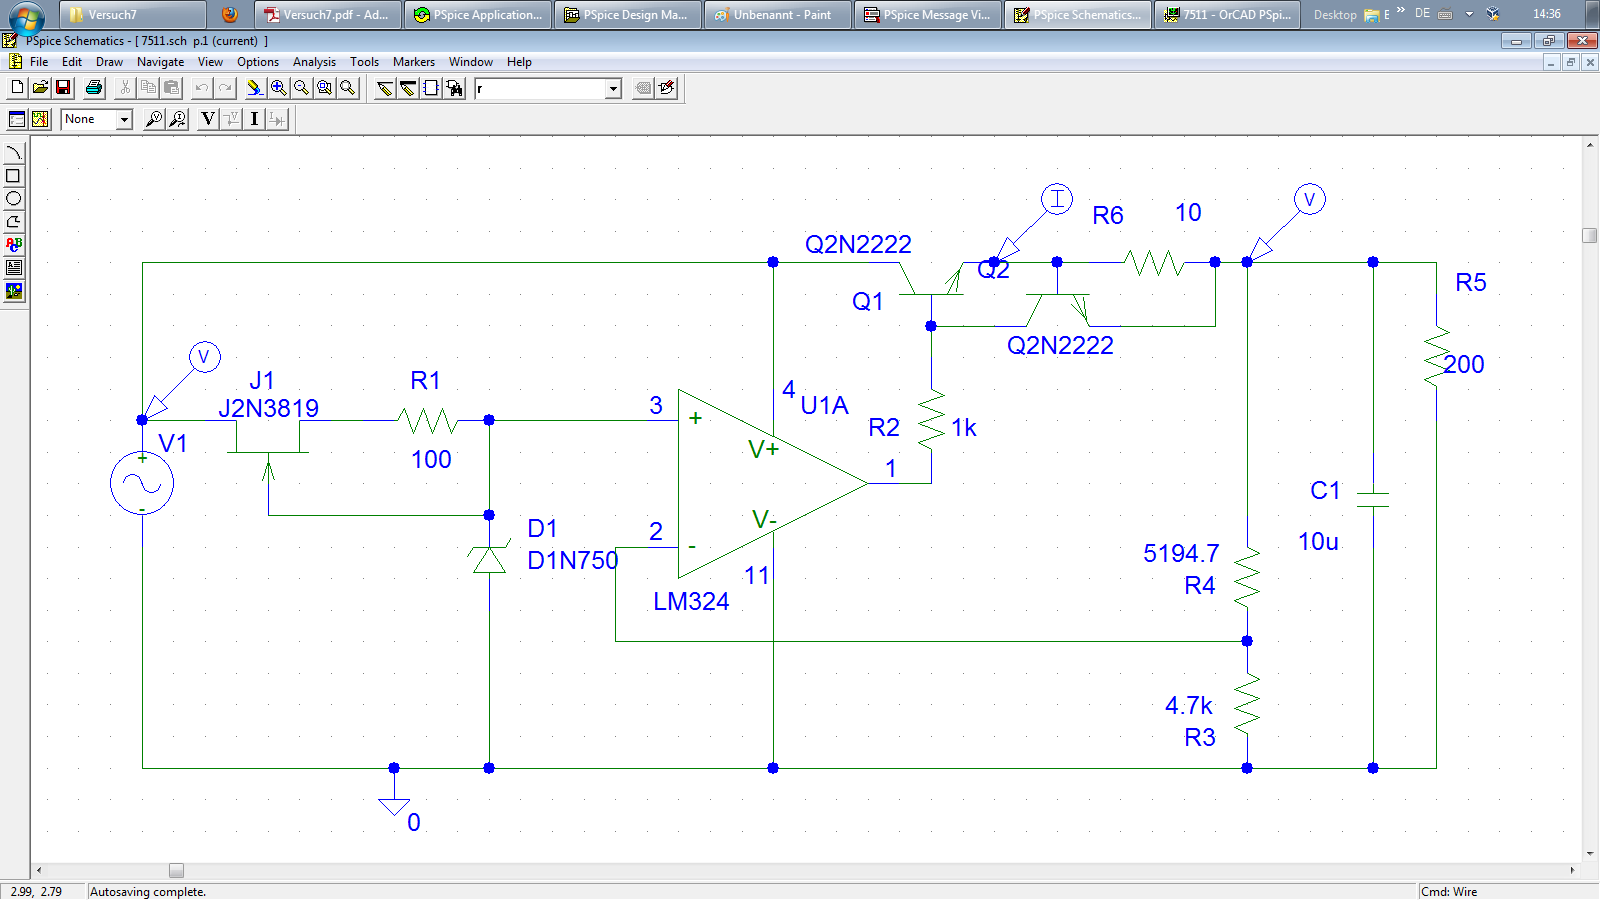
\includegraphics[width=\linewidth]{versuch7/spice/s7511.png}
	\caption{Schaltplan, wie im Skript vorgegeben}
\end{figure}
\begin{figure}[H]
	\centering
	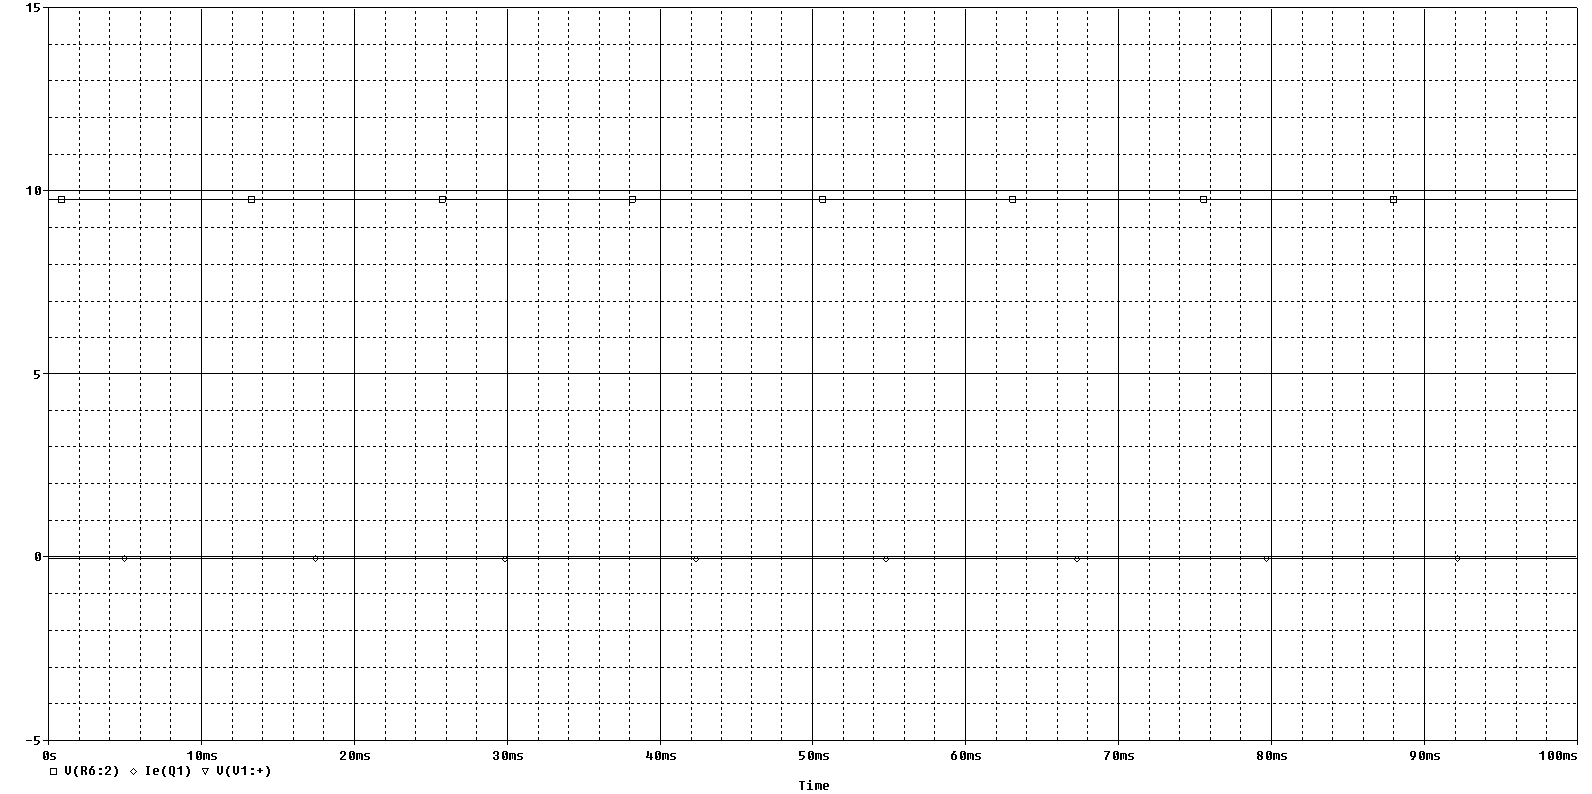
\includegraphics[width=\linewidth]{versuch7/spice/7511.png}
	\caption{Simulationsergebnis}
\end{figure}
Am Ausgang wurde bei 15V Eingangsspannung eine Spannung von 9.776V und ein Strom von 48.880mA gemessen.
Für die Güte gilt:
\[ Q=\frac{\Delta U_{EIN}}{2mV} = 2000 \]

Als nächstes wurde der Ausgang mit $ 0.1\Ohm $ kurzgeschlossen. Der Ausgangsstrom betrug nun 83.558mA bei einer Ausgangsspannung von 8.3558mV. Q2 bewirkt mit R6 eine Strombegrenzung für den Ausgang.\\
Der Ausgangsstrom ist reziprok zu $ R_6 $.\\
Die Verlustleistung beträgt: 0.071284A*14.280V = 1.0179W\\
Um die maximale Verlustleistung von 500mW nicht zu überschreiten, darf der Ausgangsstrom nicht über $ I=\frac{500mW}{15V}=0.0\overline{3}A $ gehen. Weiterhin ist der Spannungsabfall an Q6 0.712146V, mit U=RI ergibt sich somit $ R_6 = \frac{0.712146V}{0.0\overline{3}A}=21.354\Ohm $.

\subsubsection*{Messung}
Die Schaltung wurde real aufgebaut und bei 15V Eingangsspannung wurde eine Ausgangsspannung von 10.1578V gemessen. Bei 20V ergaben sich 10.1588V.
\[ \Rightarrow Q=\frac{5V}{1mV} = 5000 \]
Mit dieser Güte bin ich durchaus zufrieden.\\
Im Kurzschlussfall ergab sich ein Strom von 0.052A.






%%\vspace{\baselineskip}
%%\begin{tabular}{ll}
%%	$ R_6 $ & $ I_{out} $\\
%%	\hline
%%	5\Ohm & 154mA\\
%%	10\Ohm & 84mA\\
%%	20\Ohm & 48mA\\
%%	30\Ohm & 36mA\\
%%	40\Ohm & 30mA\\
%%	50\Ohm & 27mA\\
%%	100\Ohm & 20mA\\
%%\end{tabular}






















%}}}






%%%
%%%
%%%%{{{
%%%
%%%
%%%
%%%
%%%
%%%
%%%
%%%
%%%
%%%
%%%
%%%
%%%
%%%
%%%
%%%
%%%
%%%
%%%
%%%
%%%
%%%
%%%
%%%
%%%
%%%
%%%
%%%
%%%
%%%
%%%
%%%
%%%
%%%
%%%
%%%
%%%
%%%
%%%
%%%
%%%
%%%
%%%
%%%
%%%
%%%
%%%
%%%
%%%
%%%\subsection{Kennlinien eines Transistors}
%%%Der Vorgegebene Schaltplan wurde in Pspice eingegeben und die Simulation mit den Vorgegebenen Werten gestartet. Im Simulationsfenster wurde bei einer Kollektorspannung bestimmt:\\
%%%\begin{figure}[H]
%%%\begin{tabular}{lll}
%%%	Basistrom & Kollektorstrom & $\beta=\frac{I_C}{I_B}$ \\
%%%	\hline
%%%	 1 \µA &  121.4 \µA & 121.4\\
%%%	 2 \µA &  267.3 \µA & 133.65\\
%%%	 3 \µA &  422.6 \µA & 140.87\\
%%%	 4 \µA &  583.3 \µA & 145.82\\
%%%	 5 \µA &  748.0 \µA & 149.60\\
%%%	 6 \µA &  915.8 \µA & 152.63\\
%%%	 7 \µA & 1086.1 \µA & 155.16\\
%%%	 8 \µA & 1258.5 \µA & 157.31\\
%%%	 9 \µA & 1432.6 \µA & 159.10\\
%%%	10 \µA & 1608.3 \µA & 160.83\\
%%%\end{tabular}
%%%\caption{Kollektorstrom bei $U_{CE}=4V$}
%%%\end{figure}
%%%Damit kann man den Kollektorstrom berechnen:
%%%\[ I_B=10\µA\;\Rightarrow \; \beta=160.83;\; I_C=\beta*I_B\; \Rightarrow \; I_C=160.83*10\µA=1608.3\µA=1.6083mA \]
%%%Misst man stattdessen nach, so erhält man 1.5459mA bei 1V oder 1.6289mA bei 5V.\\
%%%Der Ausgangswiderstand berechnet sich zu:
%%%\[ R_{aus} = \frac{\Delta U_{CE}}{\Delta I_C}=\frac{5V-1V}{1.6289mA-1.5459mA}=\frac{4V}{0.083mA}=48.193k\Ohm \]
%%%
%%%\subsection{Entwurf,Simulation und Aufbau eines Transistorverstärkers (Kollektorschaltung)}
%%%Wenn man die Quelle direkt an den Verbraucher anschliest, gilt:
%%%\[ U_L = U_{Ein}*\frac{R_L}{R_i+R_L}	\]
%%%\[	U_L = U_{Ein} * \frac {R_L+\frac{1}{j*\omega*C}}{R_i+(R_L+\frac{1}{j*omega*C})}	\]
%%%\[	R_I=10k\Ohm,\; R_L=4.7k\Ohm,\; C_L=1\µF	\]
%%%Da die Frequenz bei dieser Frage nicht angegeben ist, lässt sie sich nicht genauer beantworten.\\
%%%\subsubsection*{Simulation}
%%%Die Spannungsverstärkung des Transistors ist in etwa 1, weil der Basisstrom durch die Beschaltung in etwa nur ein Hundertstel des des Emitterstroms beträgt.\\
%%%\begin{figure}[H]
%%%	\centering
%%%	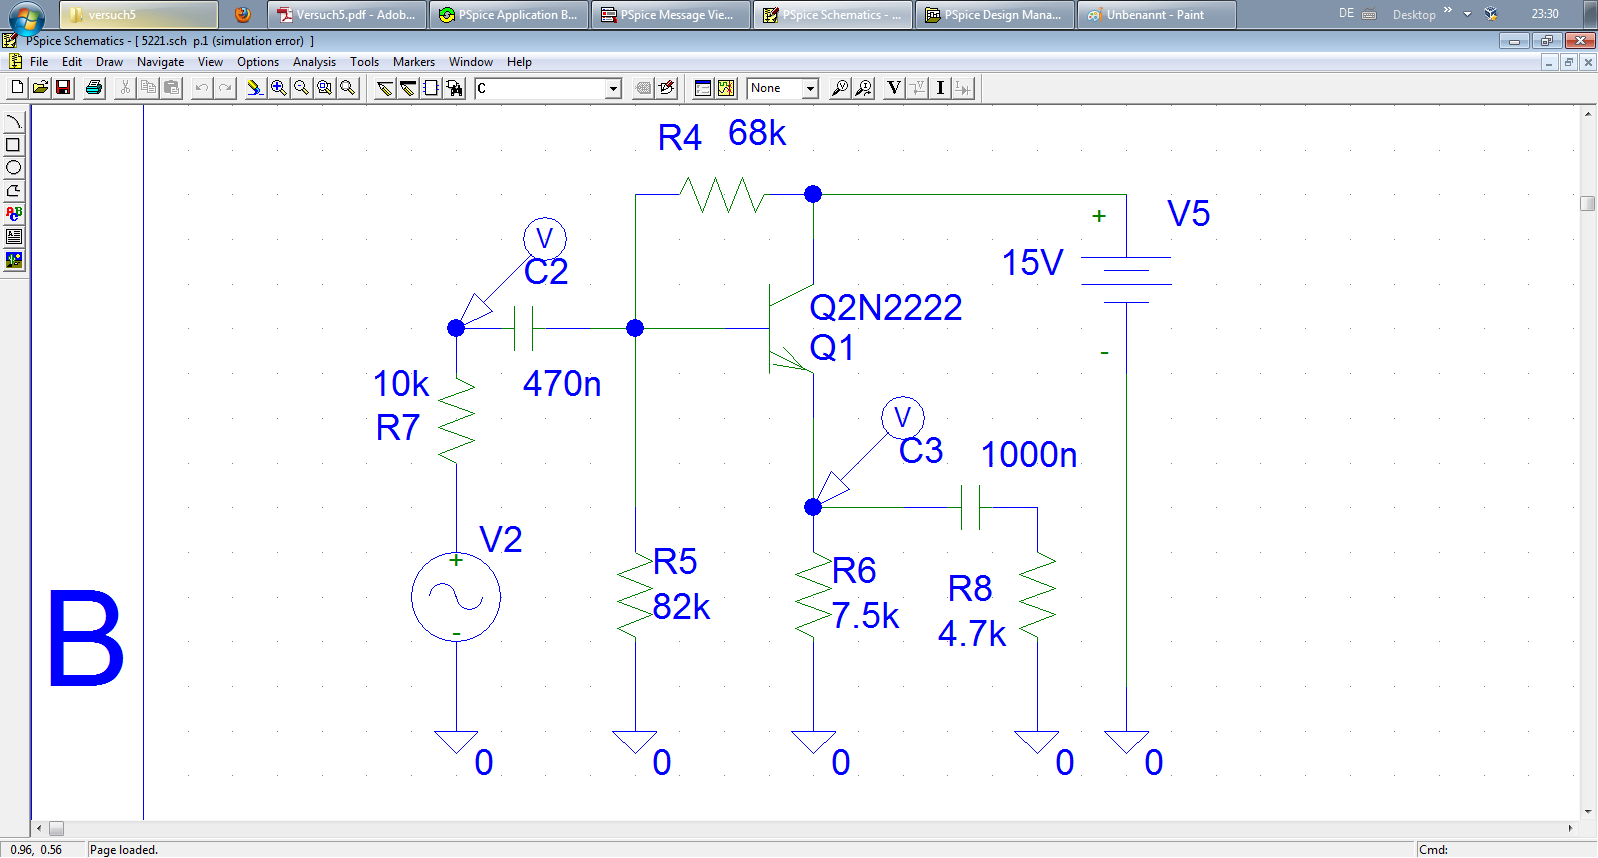
\includegraphics[width=\linewidth]{versuch5/spice/s5221.png}
%%%	\caption{Schaltplan, wie im Skript vorgegeben}
%%%\end{figure}
%%%\begin{figure}[H]
%%%	\centering
%%%	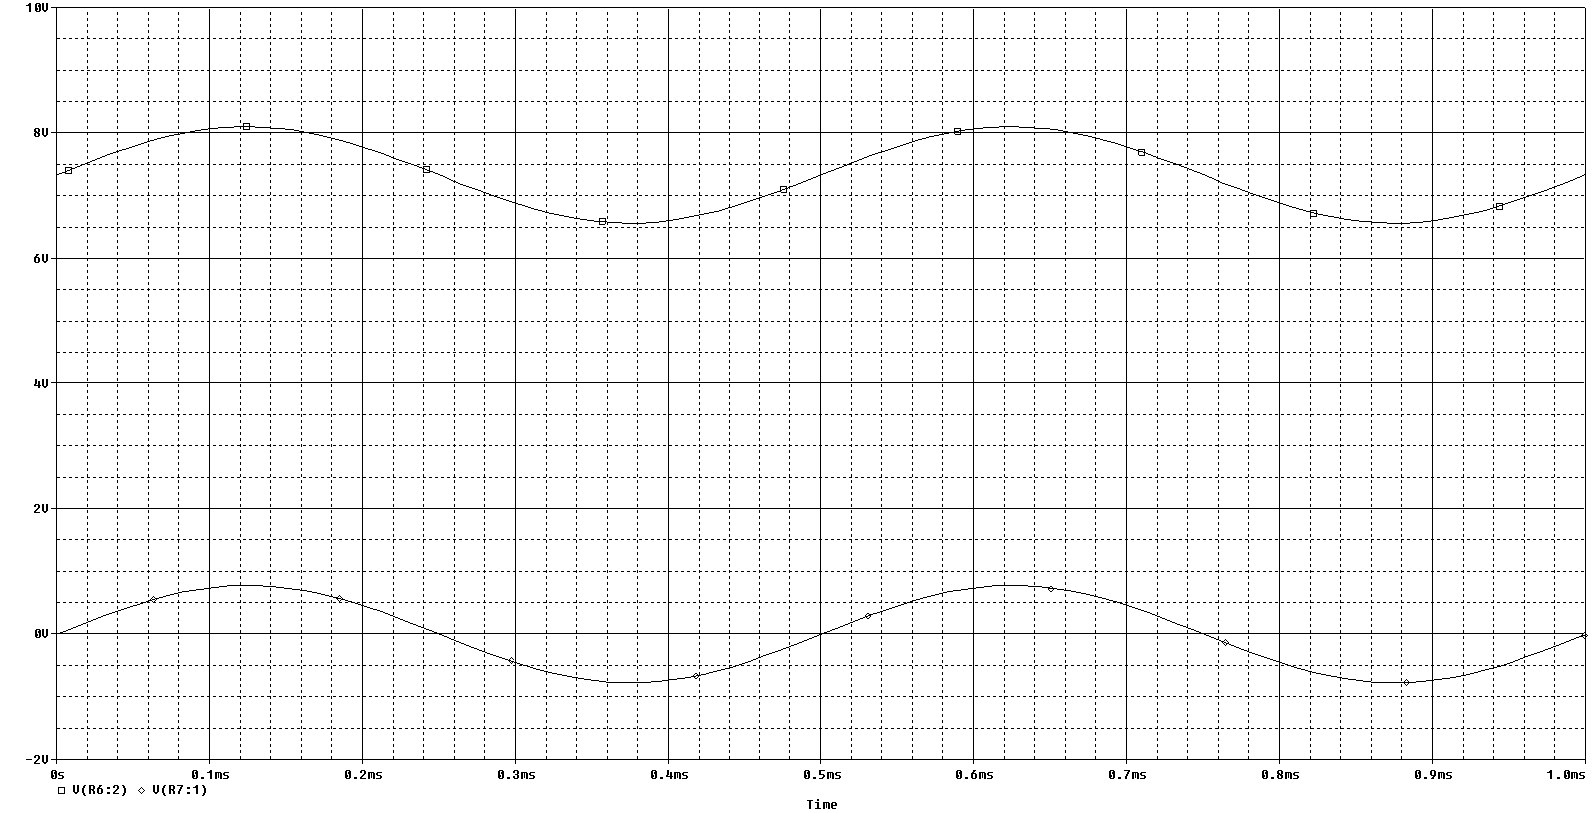
\includegraphics[width=\linewidth]{versuch5/spice/5221.png}
%%%	\caption{Simulationsergebnis}
%%%\end{figure}
%%%Als Nächstes habe ich die Amplitude auf 10V erhöht. Dabei ergab sich folgender Spannungsverlauf:
%%%\begin{figure}[H]
%%%	\centering
%%%	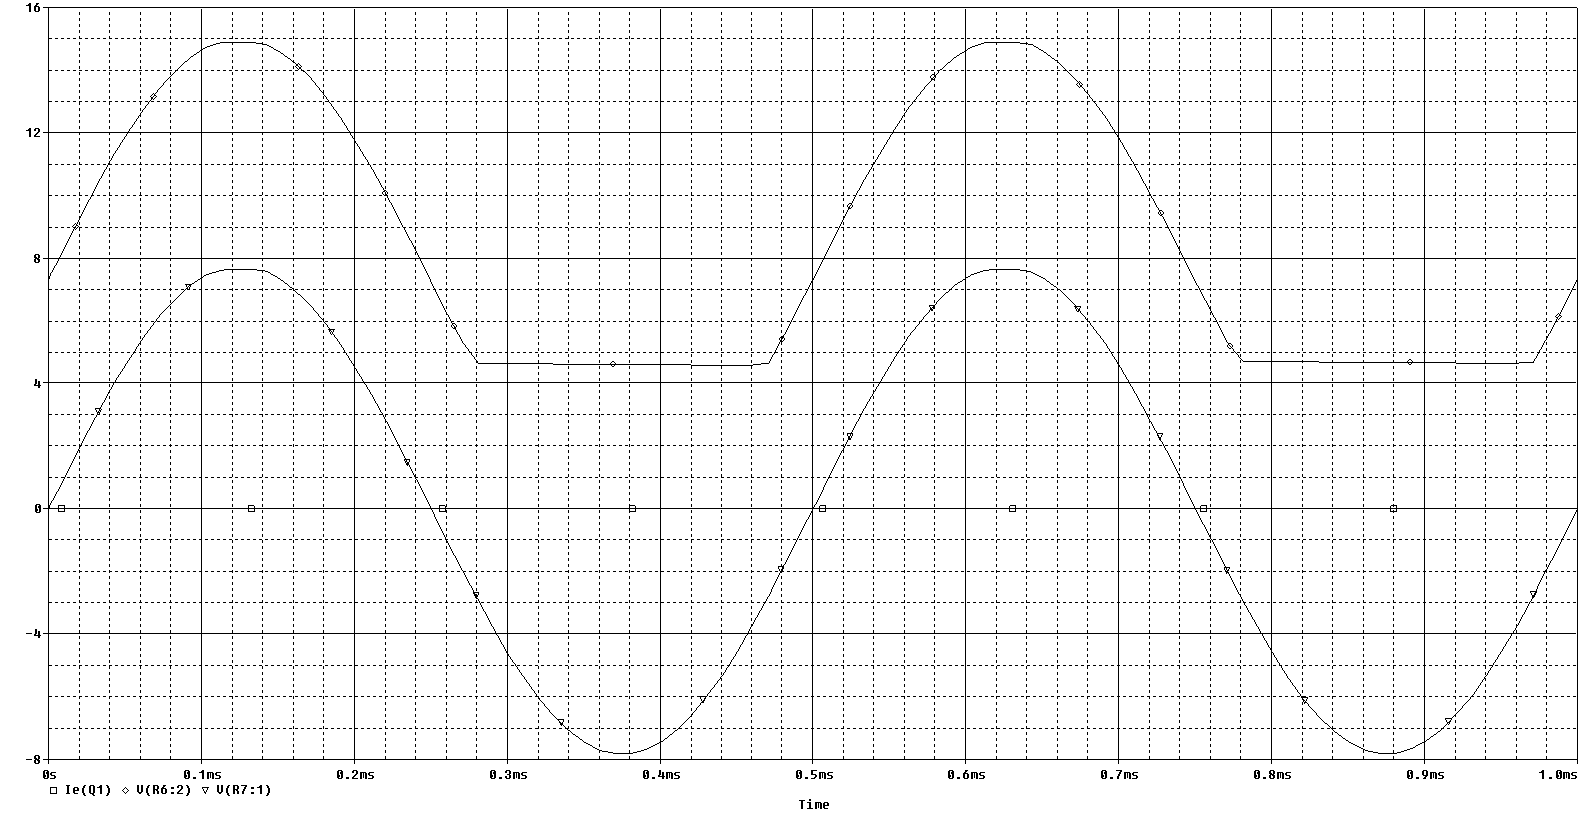
\includegraphics[width=\linewidth]{versuch5/spice/5222.png}
%%%	\caption{Simulationsergebnis}
%%%\end{figure}
%%%\begin{figure}[H]
%%%	\centering
%%%	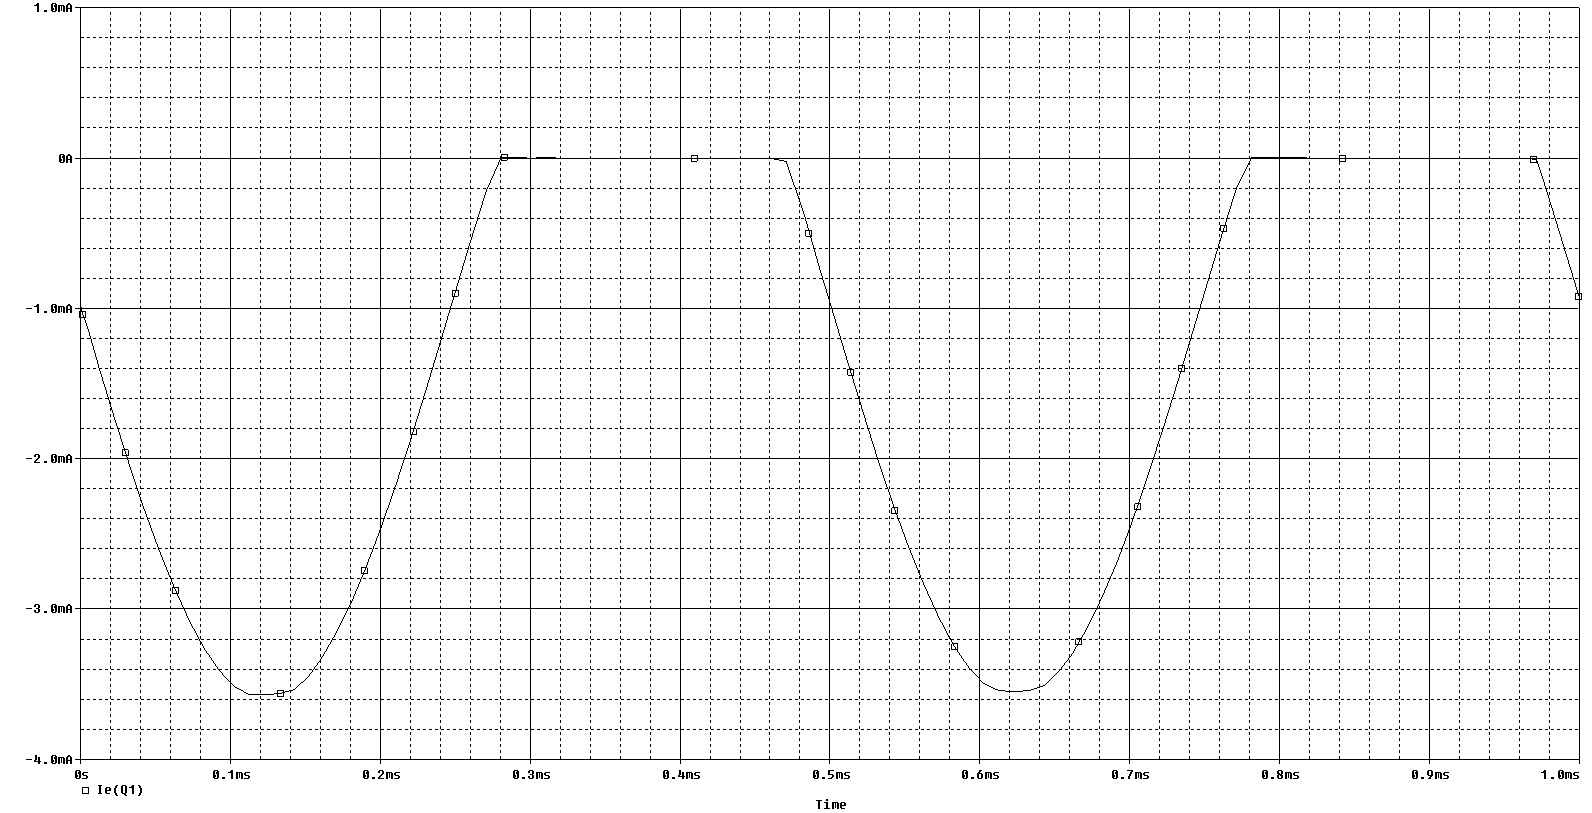
\includegraphics[width=\linewidth]{versuch5/spice/5222I.png}
%%%	\caption{Simulationsergebnis: Nur Strom}
%%%\end{figure}
%%%Es zeigen sich deutlich die Clipping-Effekte bei einer Ausgangsspannung unterhalb 4.65V.\\
%%%Dieser Effekt rührt daher, dass der Kondensator C3 das Spannungsnieveau hält. bei den 4.65V trifft die (steigende) Ladekurve des Kondensators auf die (fallende) Spannungskurve des variablen Widerstandsteilers aus Q1 und R6, daher erscheint ein deutlich sichtbarer Knick im Verlauf der Ausgangsspannung. Um die Spannung auch auf der negativen Halbwelle tiefer einstellen zu können müsste R6 kleiner gewählt sein (mit allen Folgen), oder man verwendet gleich auch einen Transistor, dann lässt sich auch eine kapazitive Last mit weniger Verzerrungen ansteuern.
%%%
%%%Bei niedrigen Frequenzen dominiert die Hochpasscharakteristik des Filters aus R7, C2 und R5. Das Eingangssignal wird also vom Filter gedämpft, daher wird der Transistor nicht voll angesteuert und somit ist die Verstärkung insgesammt eher schwach, obwohl der Transistor an sich mit den niedrigen Frequenzen kein Problem hätte.\\
%%%Die Amplitude des Eingangssignals steigt bei niedrigen Frequenzen an, weil der Kondensator dort hochohmig(-er) ist. Somit wird die Reale Spannungsquelle aus V2 und R7 schwächer belastet und kommt somit iher Leerlaufspannung näher.
%%%\subsubsection*{Messung}
%%%Die aufgebaute Platine lieferte folgende Ausgangsspannung:
%%%\begin{figure}[H]
%%%	\centering
%%%	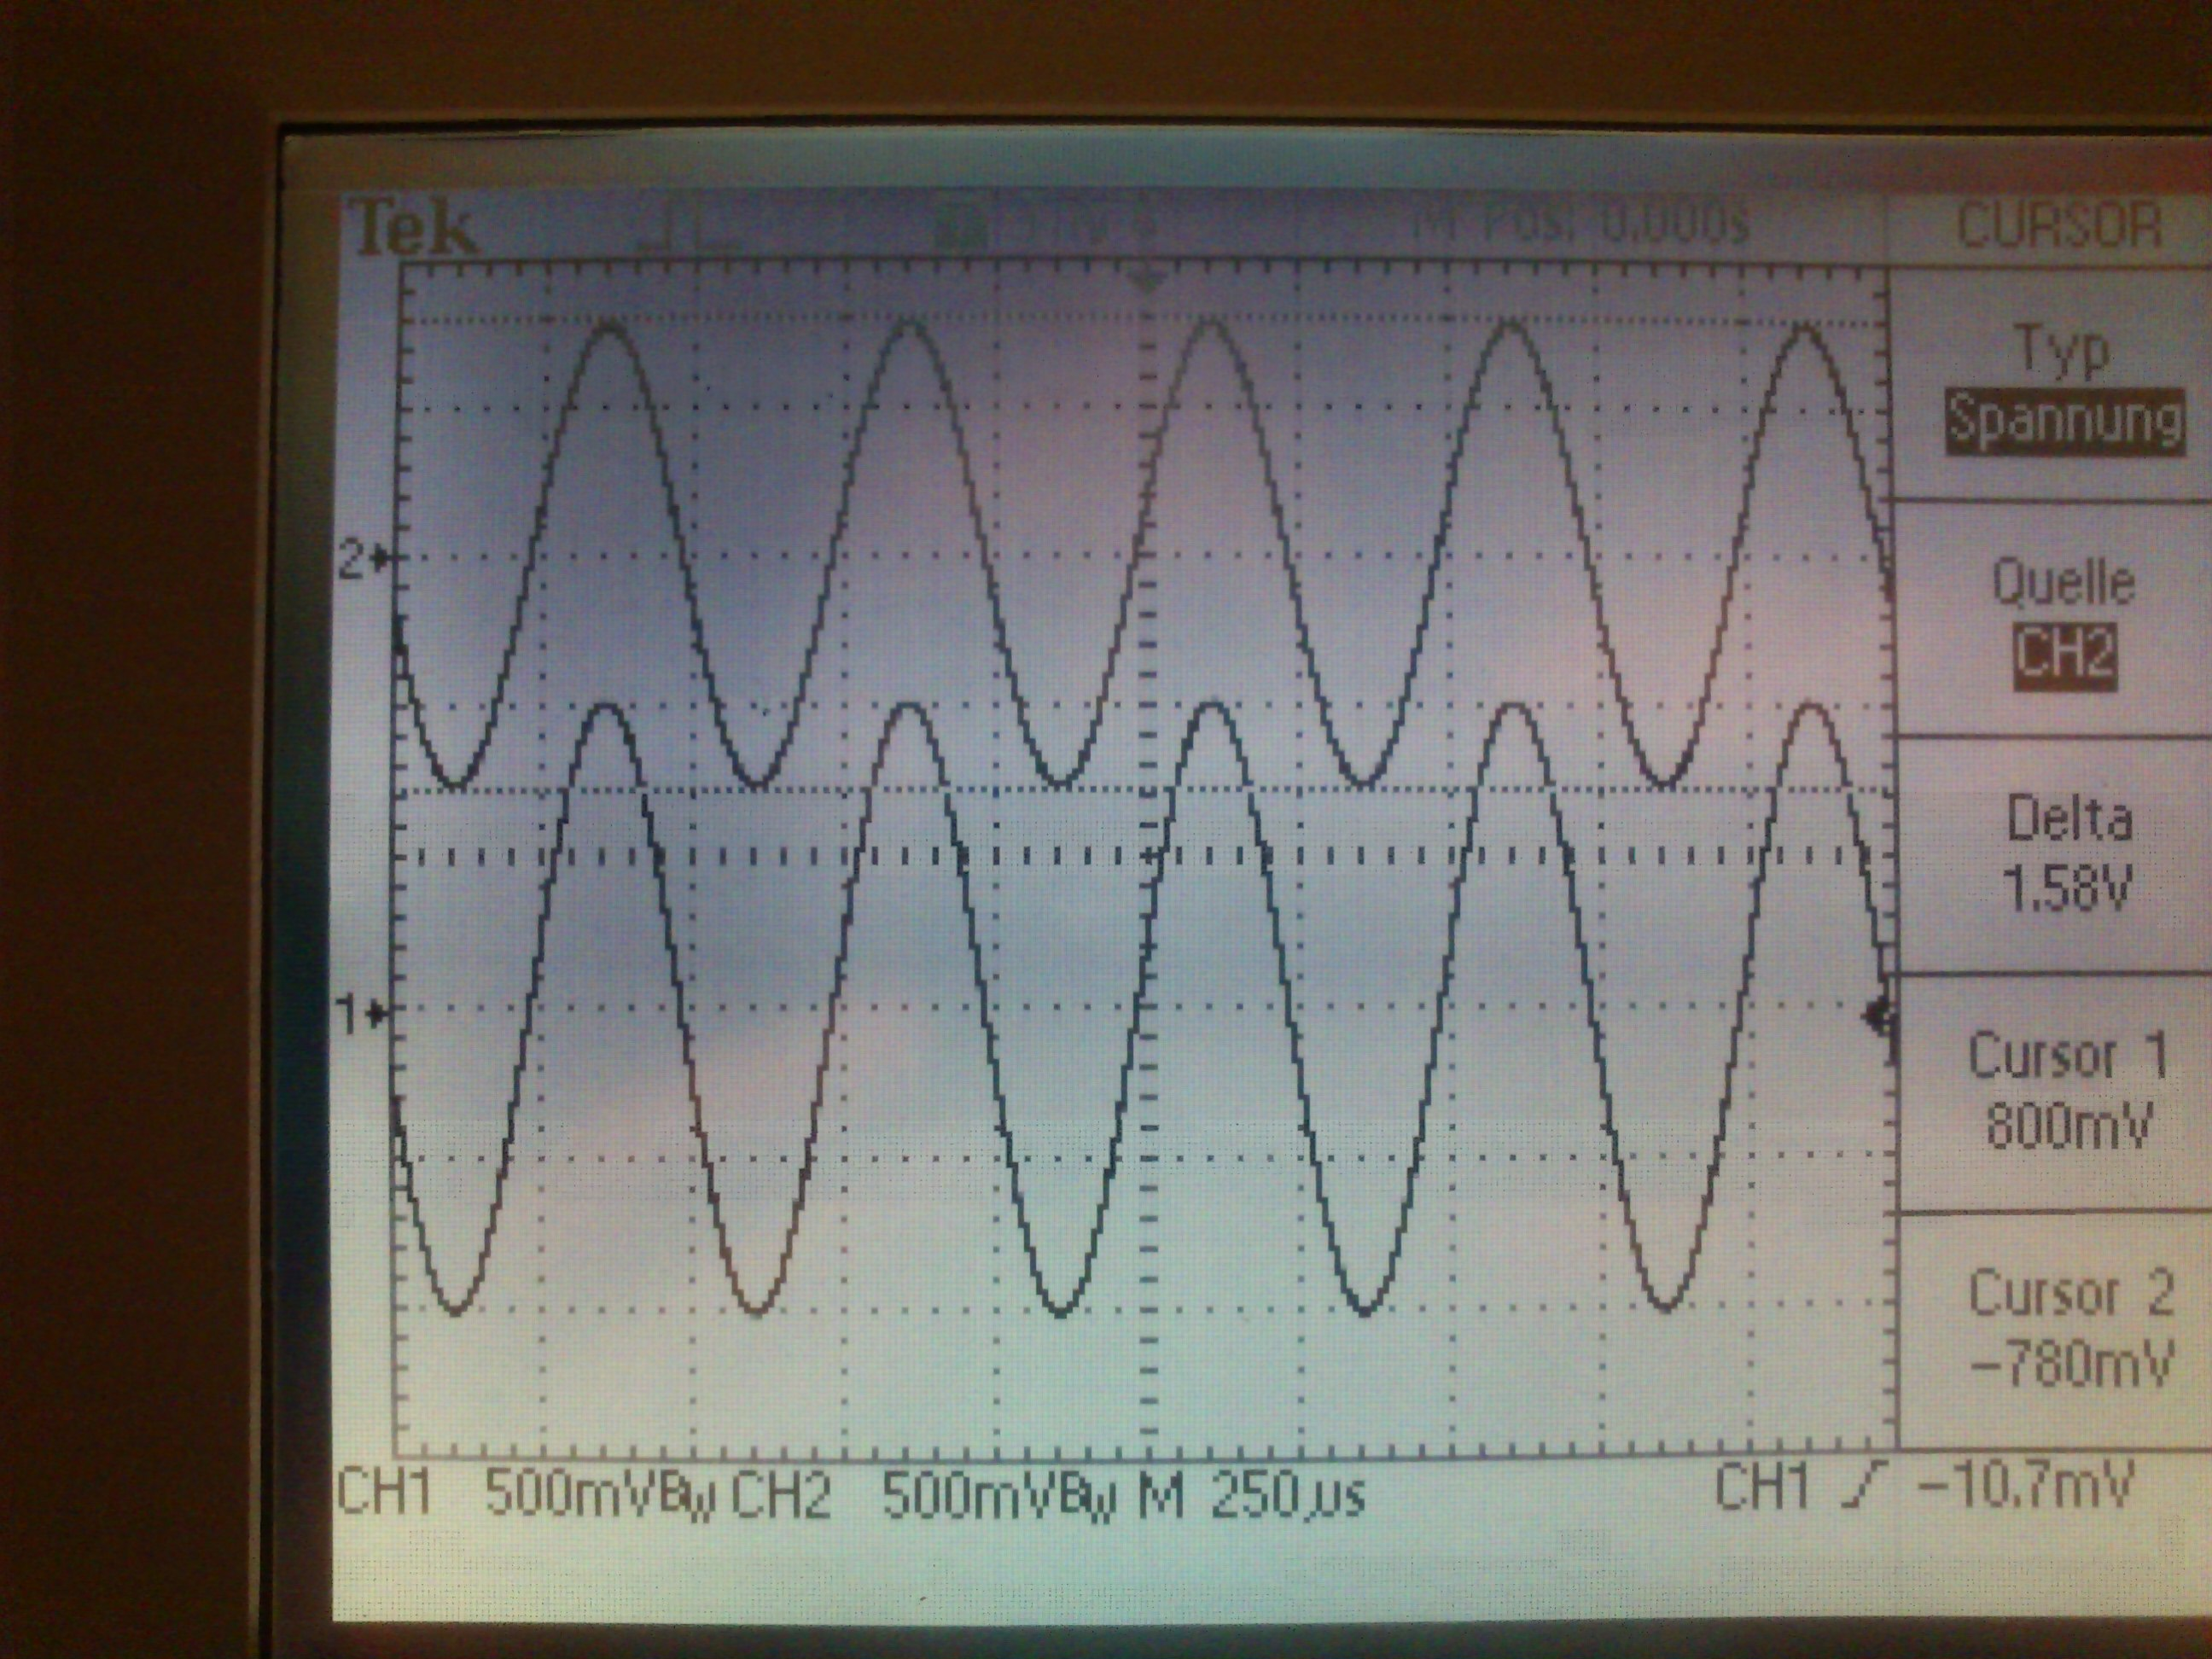
\includegraphics[width=\linewidth]{versuch5/oszi/DSC_0444.JPG}
%%%	\caption{Ausgangsspannung bei 2kHz: 1.58V, Eingangsspannung: 1.02V}
%%%\end{figure}
%%%Die reale Schaltung liefert mehr Spannung als erwartet. Es ergibt sich somit ein Verstärkungsfaktor von $\frac{1.58}{1.02}=1.549\approx1.55$.
%%%
%%%
%%%\subsection{Entwurf, Simulation und Aufbau eines Transistorverstärkers (Emitterschaltung)}
%%%\subsubsection*{Simulation}
%%%Die Bauteilwerte wurden wie folgt bestimmt:\\
%%%\begin{tabular}{ll}
%%%	Bauteil & Wert\\
%%%	\hline
%%%	C1 & 79.6nF, verwendet 220nF\\
%%%	C2 & 9.3 \mikro F, verwendet 22 \µF\\
%%%	R1 & 100k\Ohm\\
%%%	R2 & 8.2k\Ohm, verwendet: 9.1k\Ohm\\
%%%	R3 & 171.43\Ohm\\
%%%	RC & 20k\Ohm\\
%%%	RE & 2k\Ohm\\
%%%\end{tabular}
%%%
%%%\begin{figure}[H]
%%%	\centering
%%%	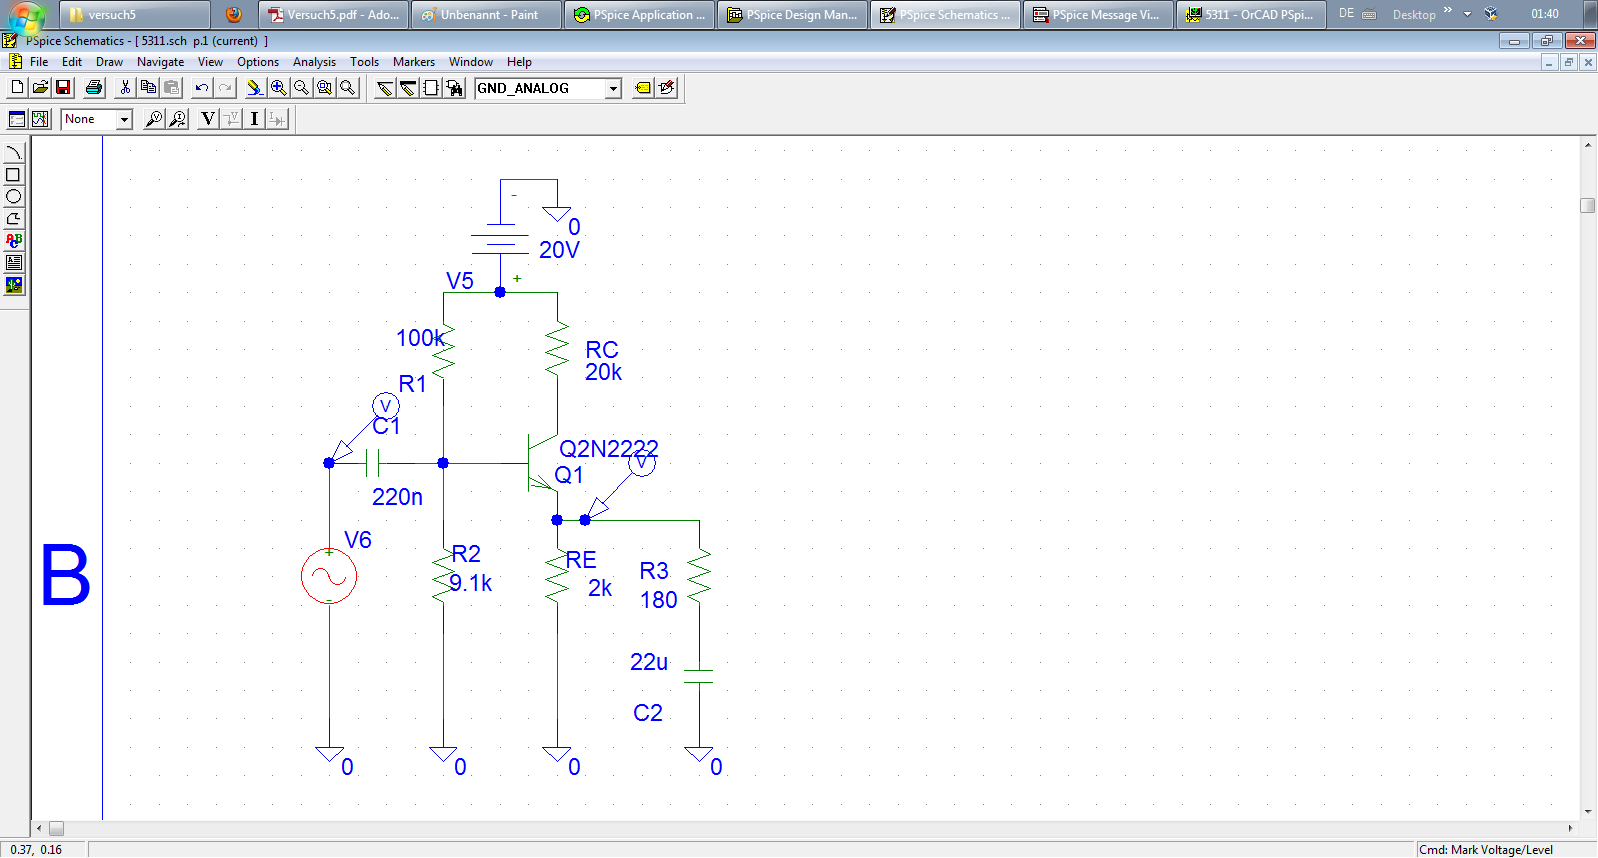
\includegraphics[width=\linewidth]{versuch5/spice/s5312.png}
%%%	\caption{Schaltplan, wie im Skript vorgegeben}
%%%\end{figure}
%%%\begin{figure}[H]
%%%	\centering
%%%	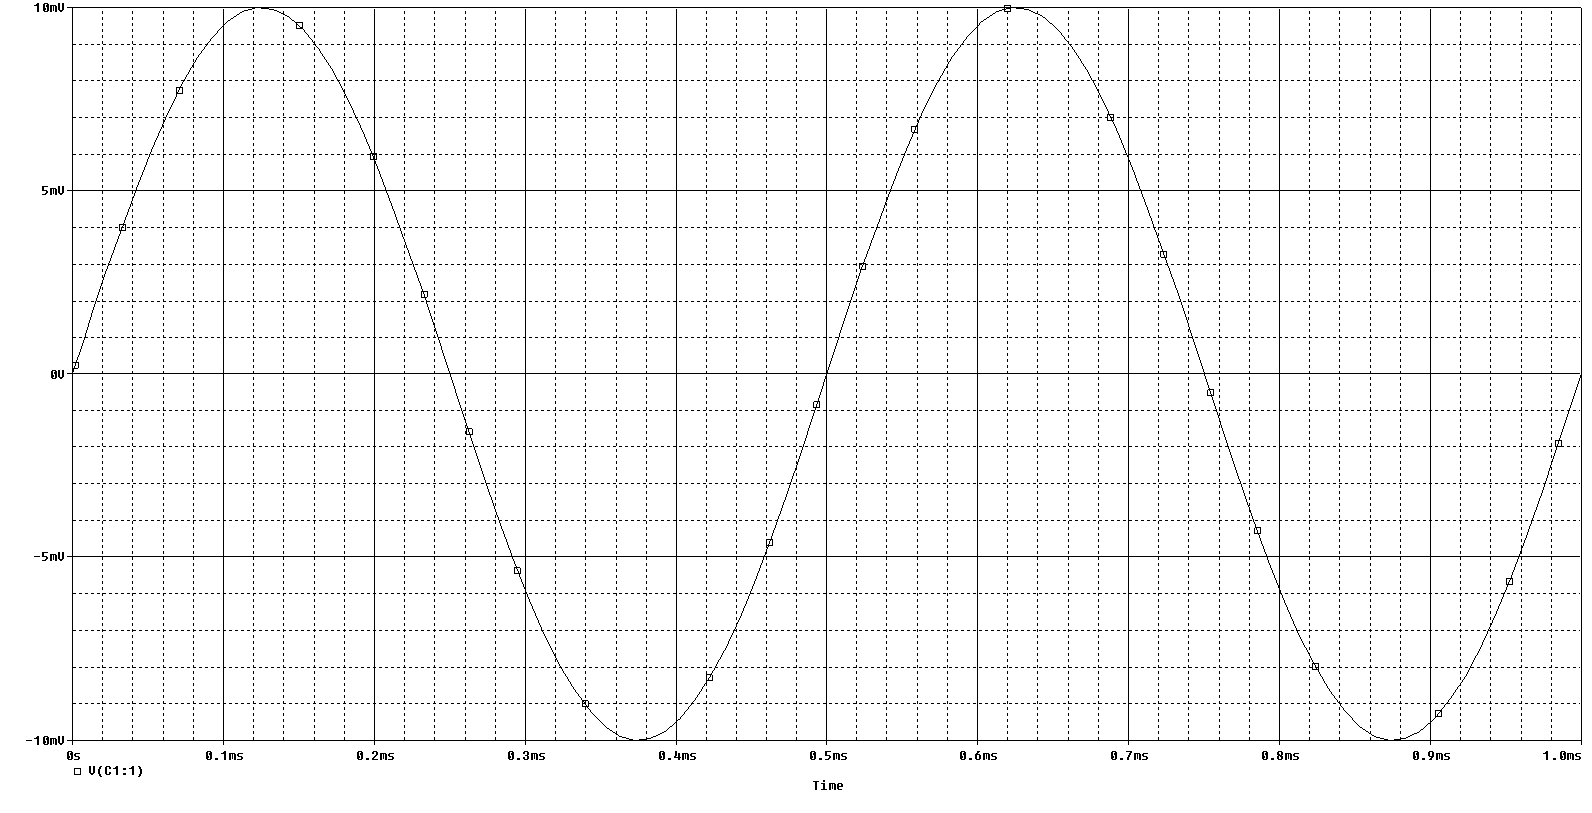
\includegraphics[width=\linewidth]{versuch5/spice/5311e.png}
%%%	\caption{Simulationsergebnis: Eingangsspannung}
%%%\end{figure}
%%%\begin{figure}[H]
%%%	\centering
%%%	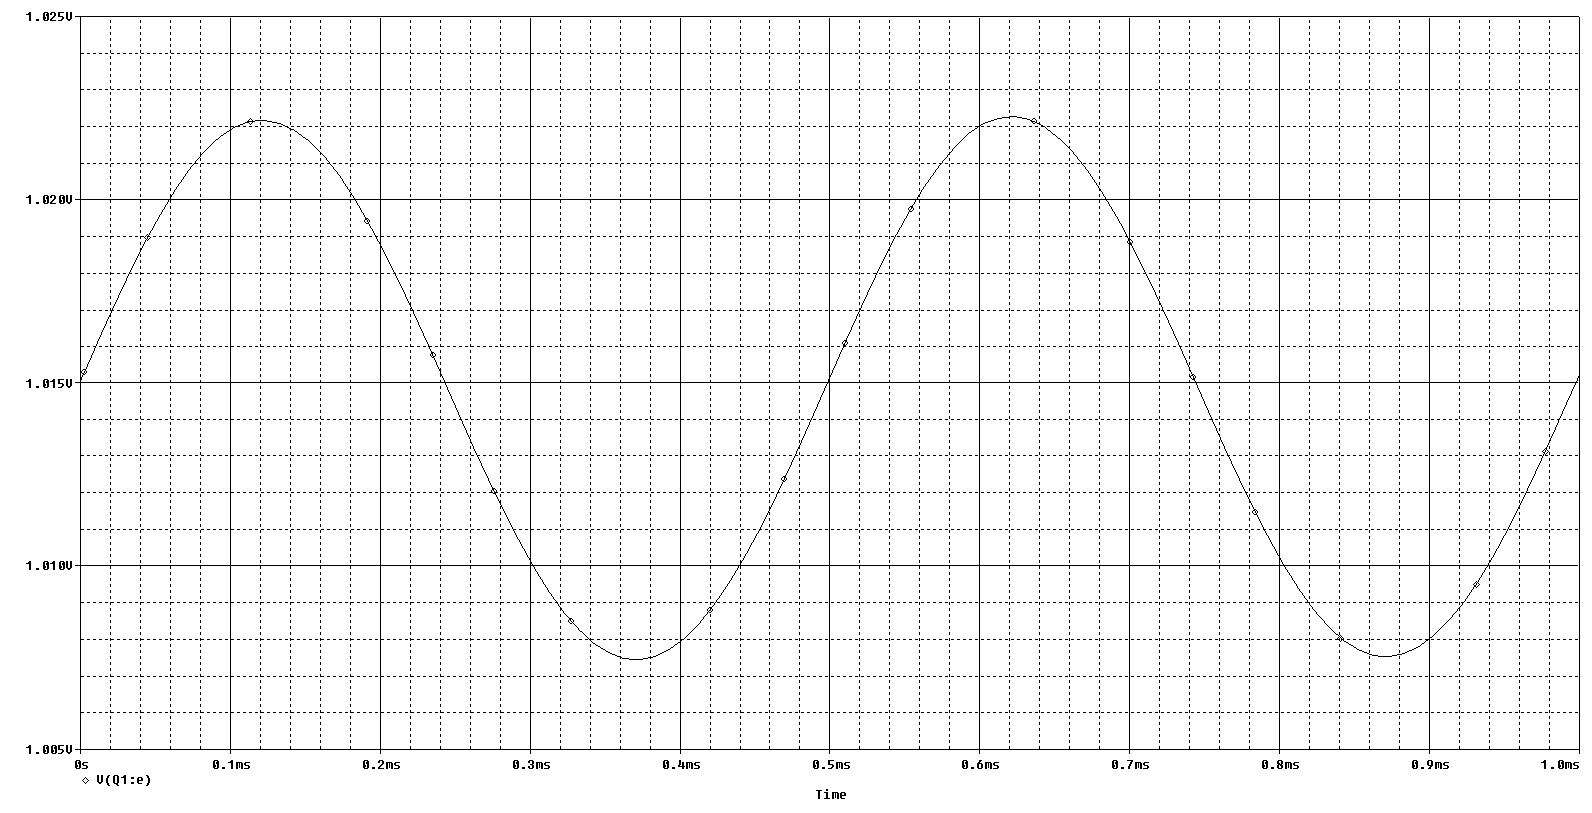
\includegraphics[width=\linewidth]{versuch5/spice/5311a.png}
%%%	\caption{Simulationsergebnis: Ausgangsspannung}
%%%\end{figure}
%%%Die simulierte Verstärkung ist $\frac{1.22}{0.01}=122$.\\
%%%Als nächstes habe ich die Amplitude der Signalquelle verzehnfacht:
%%%\begin{figure}[H]
%%%	\centering
%%%	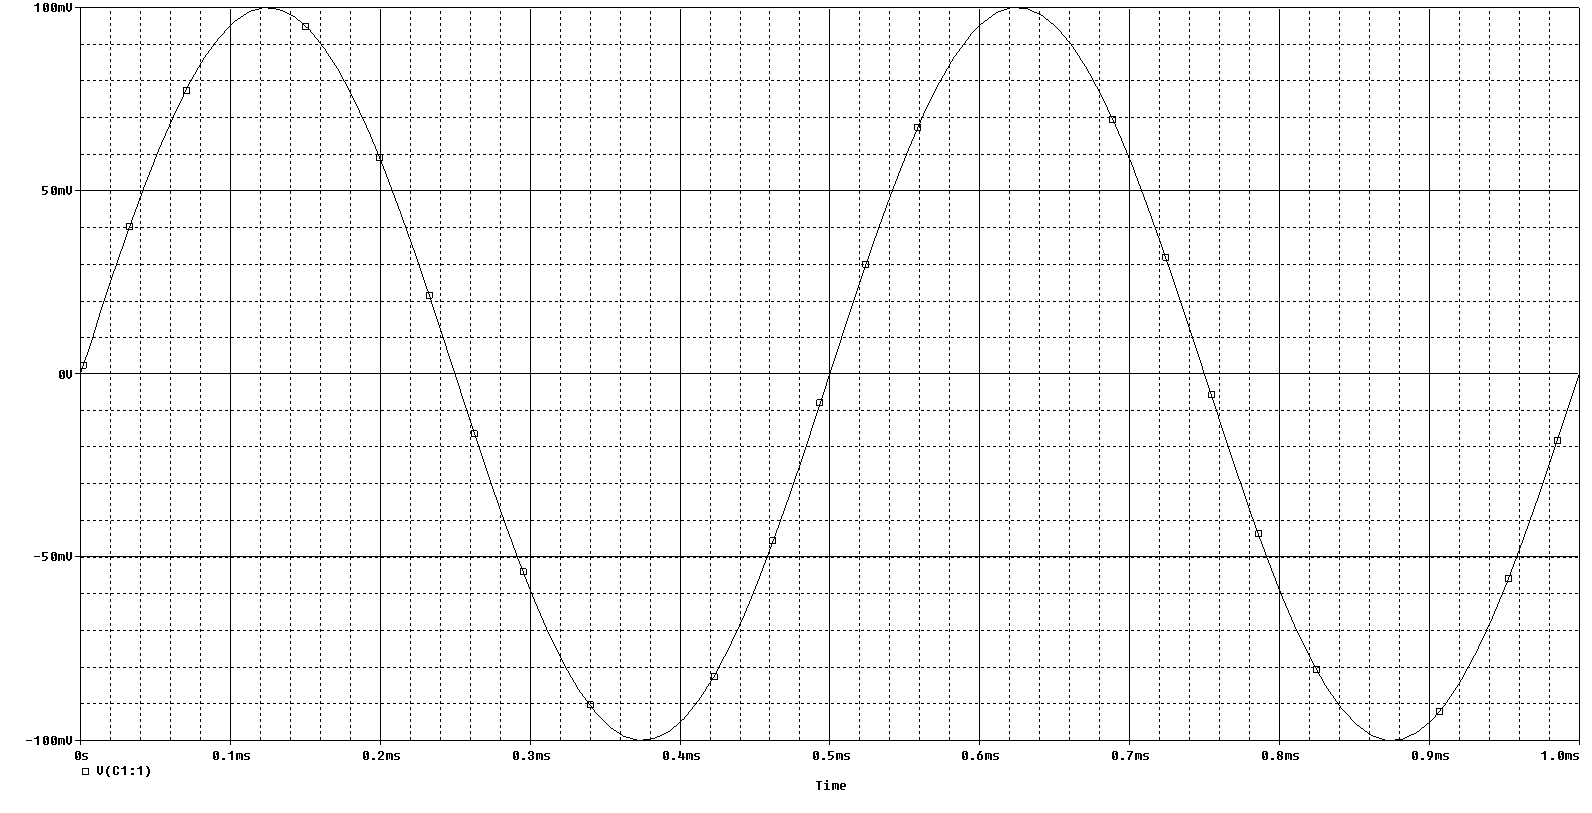
\includegraphics[width=\linewidth]{versuch5/spice/5312e.png}
%%%	\caption{Simulationsergebnis: Eingangsspannung}
%%%\end{figure}
%%%\begin{figure}[H]
%%%	\centering
%%%	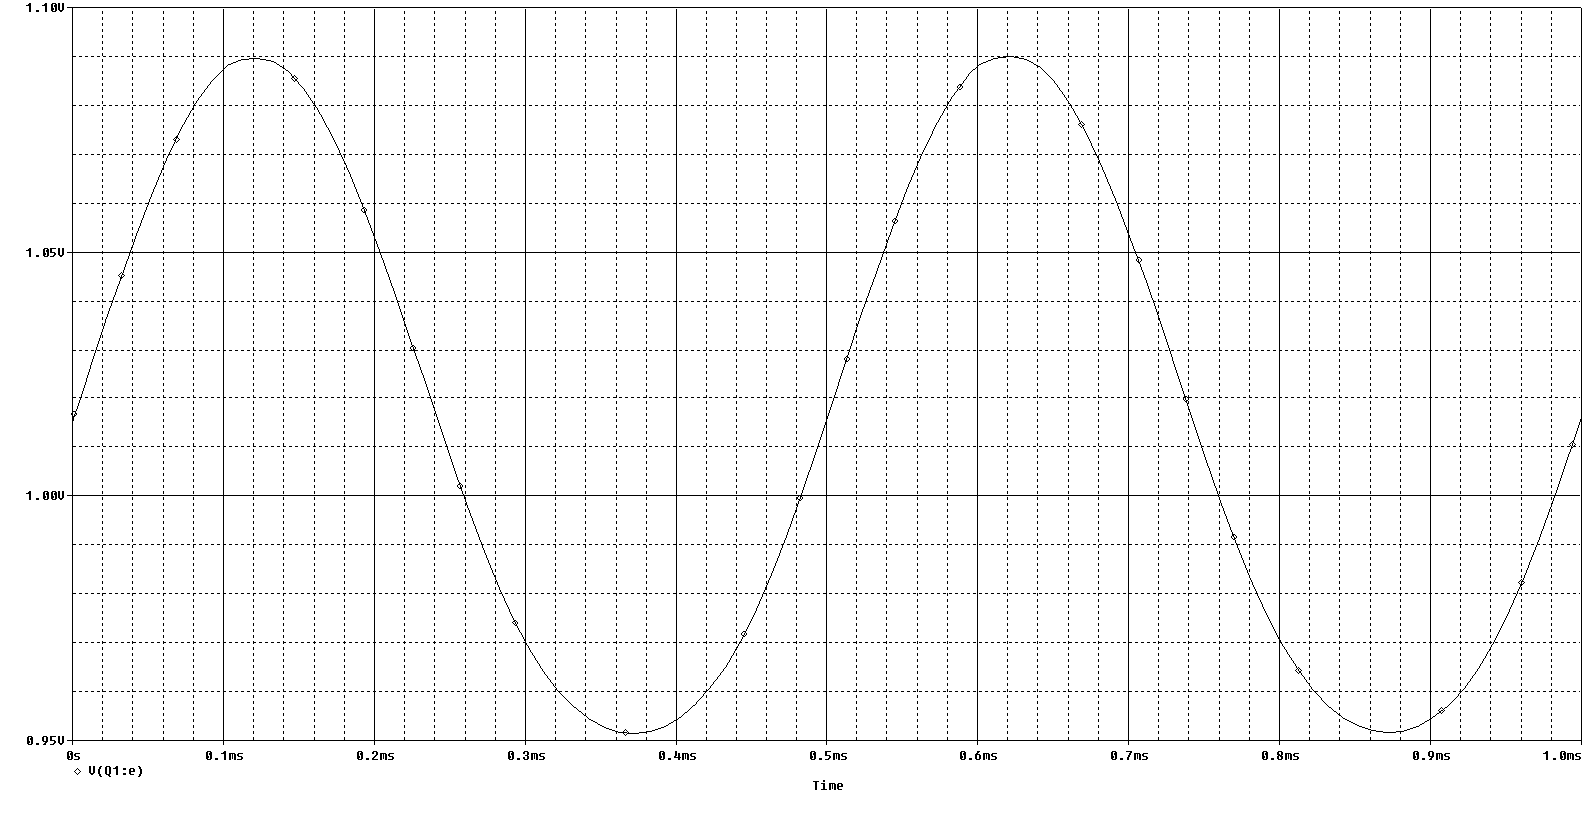
\includegraphics[width=\linewidth]{versuch5/spice/5312a.png}
%%%	\caption{Simulationsergebnis: Ausgangsspannung}
%%%\end{figure}
%%%Man sieht deutlich, dass der Mittelwert des Ausgangssignals durch die Bezugspunktverschiebung des Transistors nach oben verschoben wurde. Die Verzerrungen wurden noch im Frequenzbereich untersucht:
%%%\begin{figure}[H]
%%%	\centering
%%%	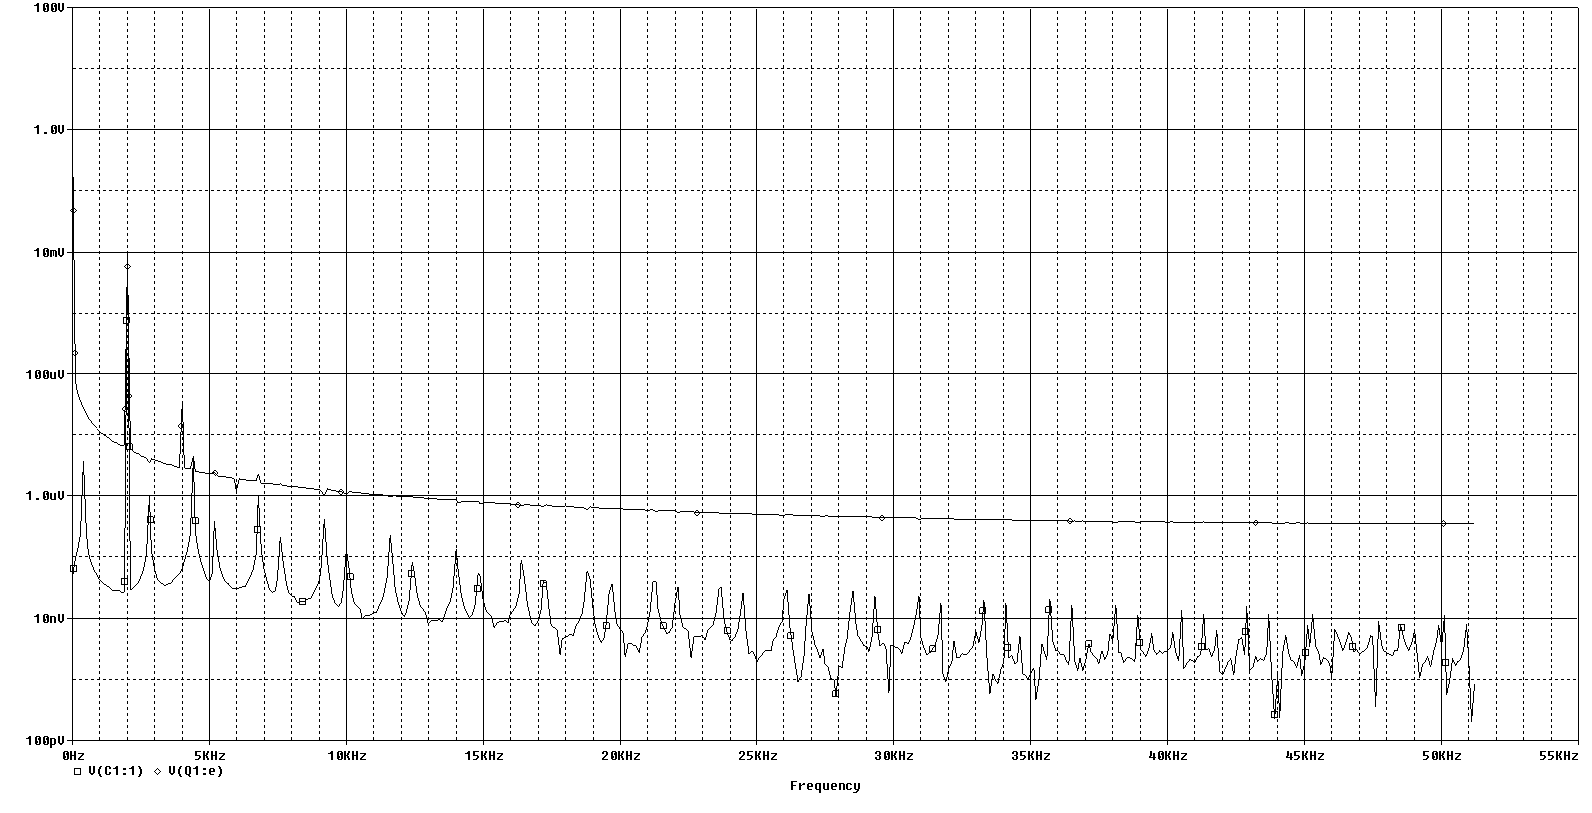
\includegraphics[width=\linewidth]{versuch5/spice/5313f1.png}
%%%	\caption{Simulationsergebnis bei 10mV Eingangsspannung}
%%%\end{figure}
%%%\begin{figure}[H]
%%%	\centering
%%%	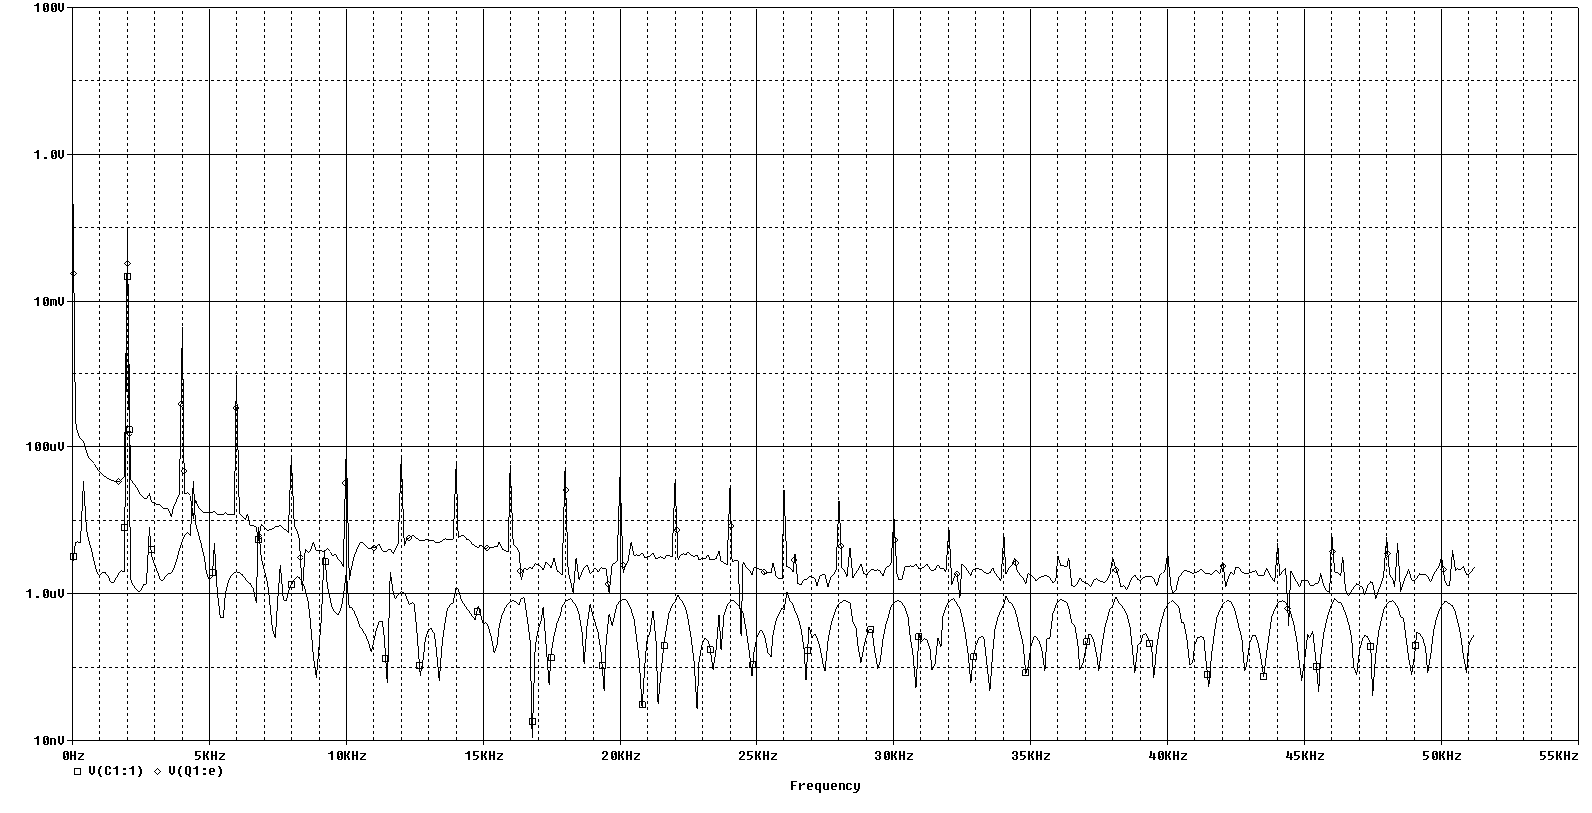
\includegraphics[width=\linewidth]{versuch5/spice/5313f2.png}
%%%	\caption{Simulationsergebnis bei 100mV Eingangsspannung}
%%%\end{figure}
%%%Die Spitzenwerte der Oberwellen sind: 70mV, 45mV, 510\µ V, 100\µ V, 100\µ V. Daraus ergibt sich der Klirrfaktor wie folgt:
%%%\[ \sqrt{\frac{\sum_{k=2}^5U_k^2}{\sum_{k=1}^5U_k^2}}=0.54 \]
%%%Dann führte ich noch einen AC-Sweep aus:
%%%\begin{figure}[H]
%%%	\centering
%%%	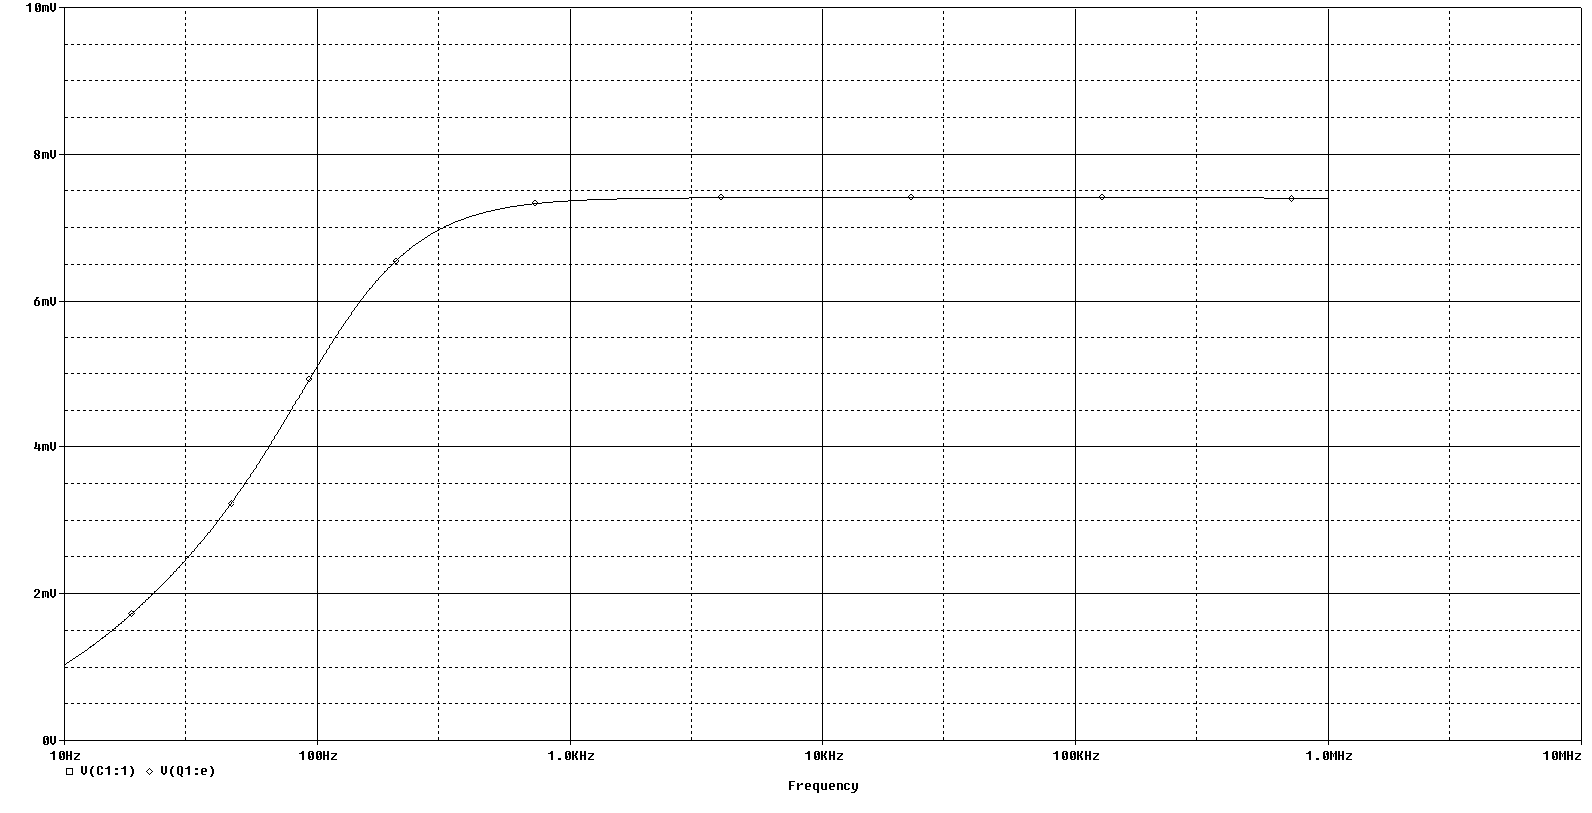
\includegraphics[width=\linewidth]{versuch5/spice/5314.png}
%%%	\caption{Simulationsergebnis Ausgangsspannung im Abhängigkeit der Frequenz}
%%%\end{figure}
%%%
%%%
%%%\subsubsection*{Messung}
%%%\begin{figure}[H]
%%%	\centering
%%%	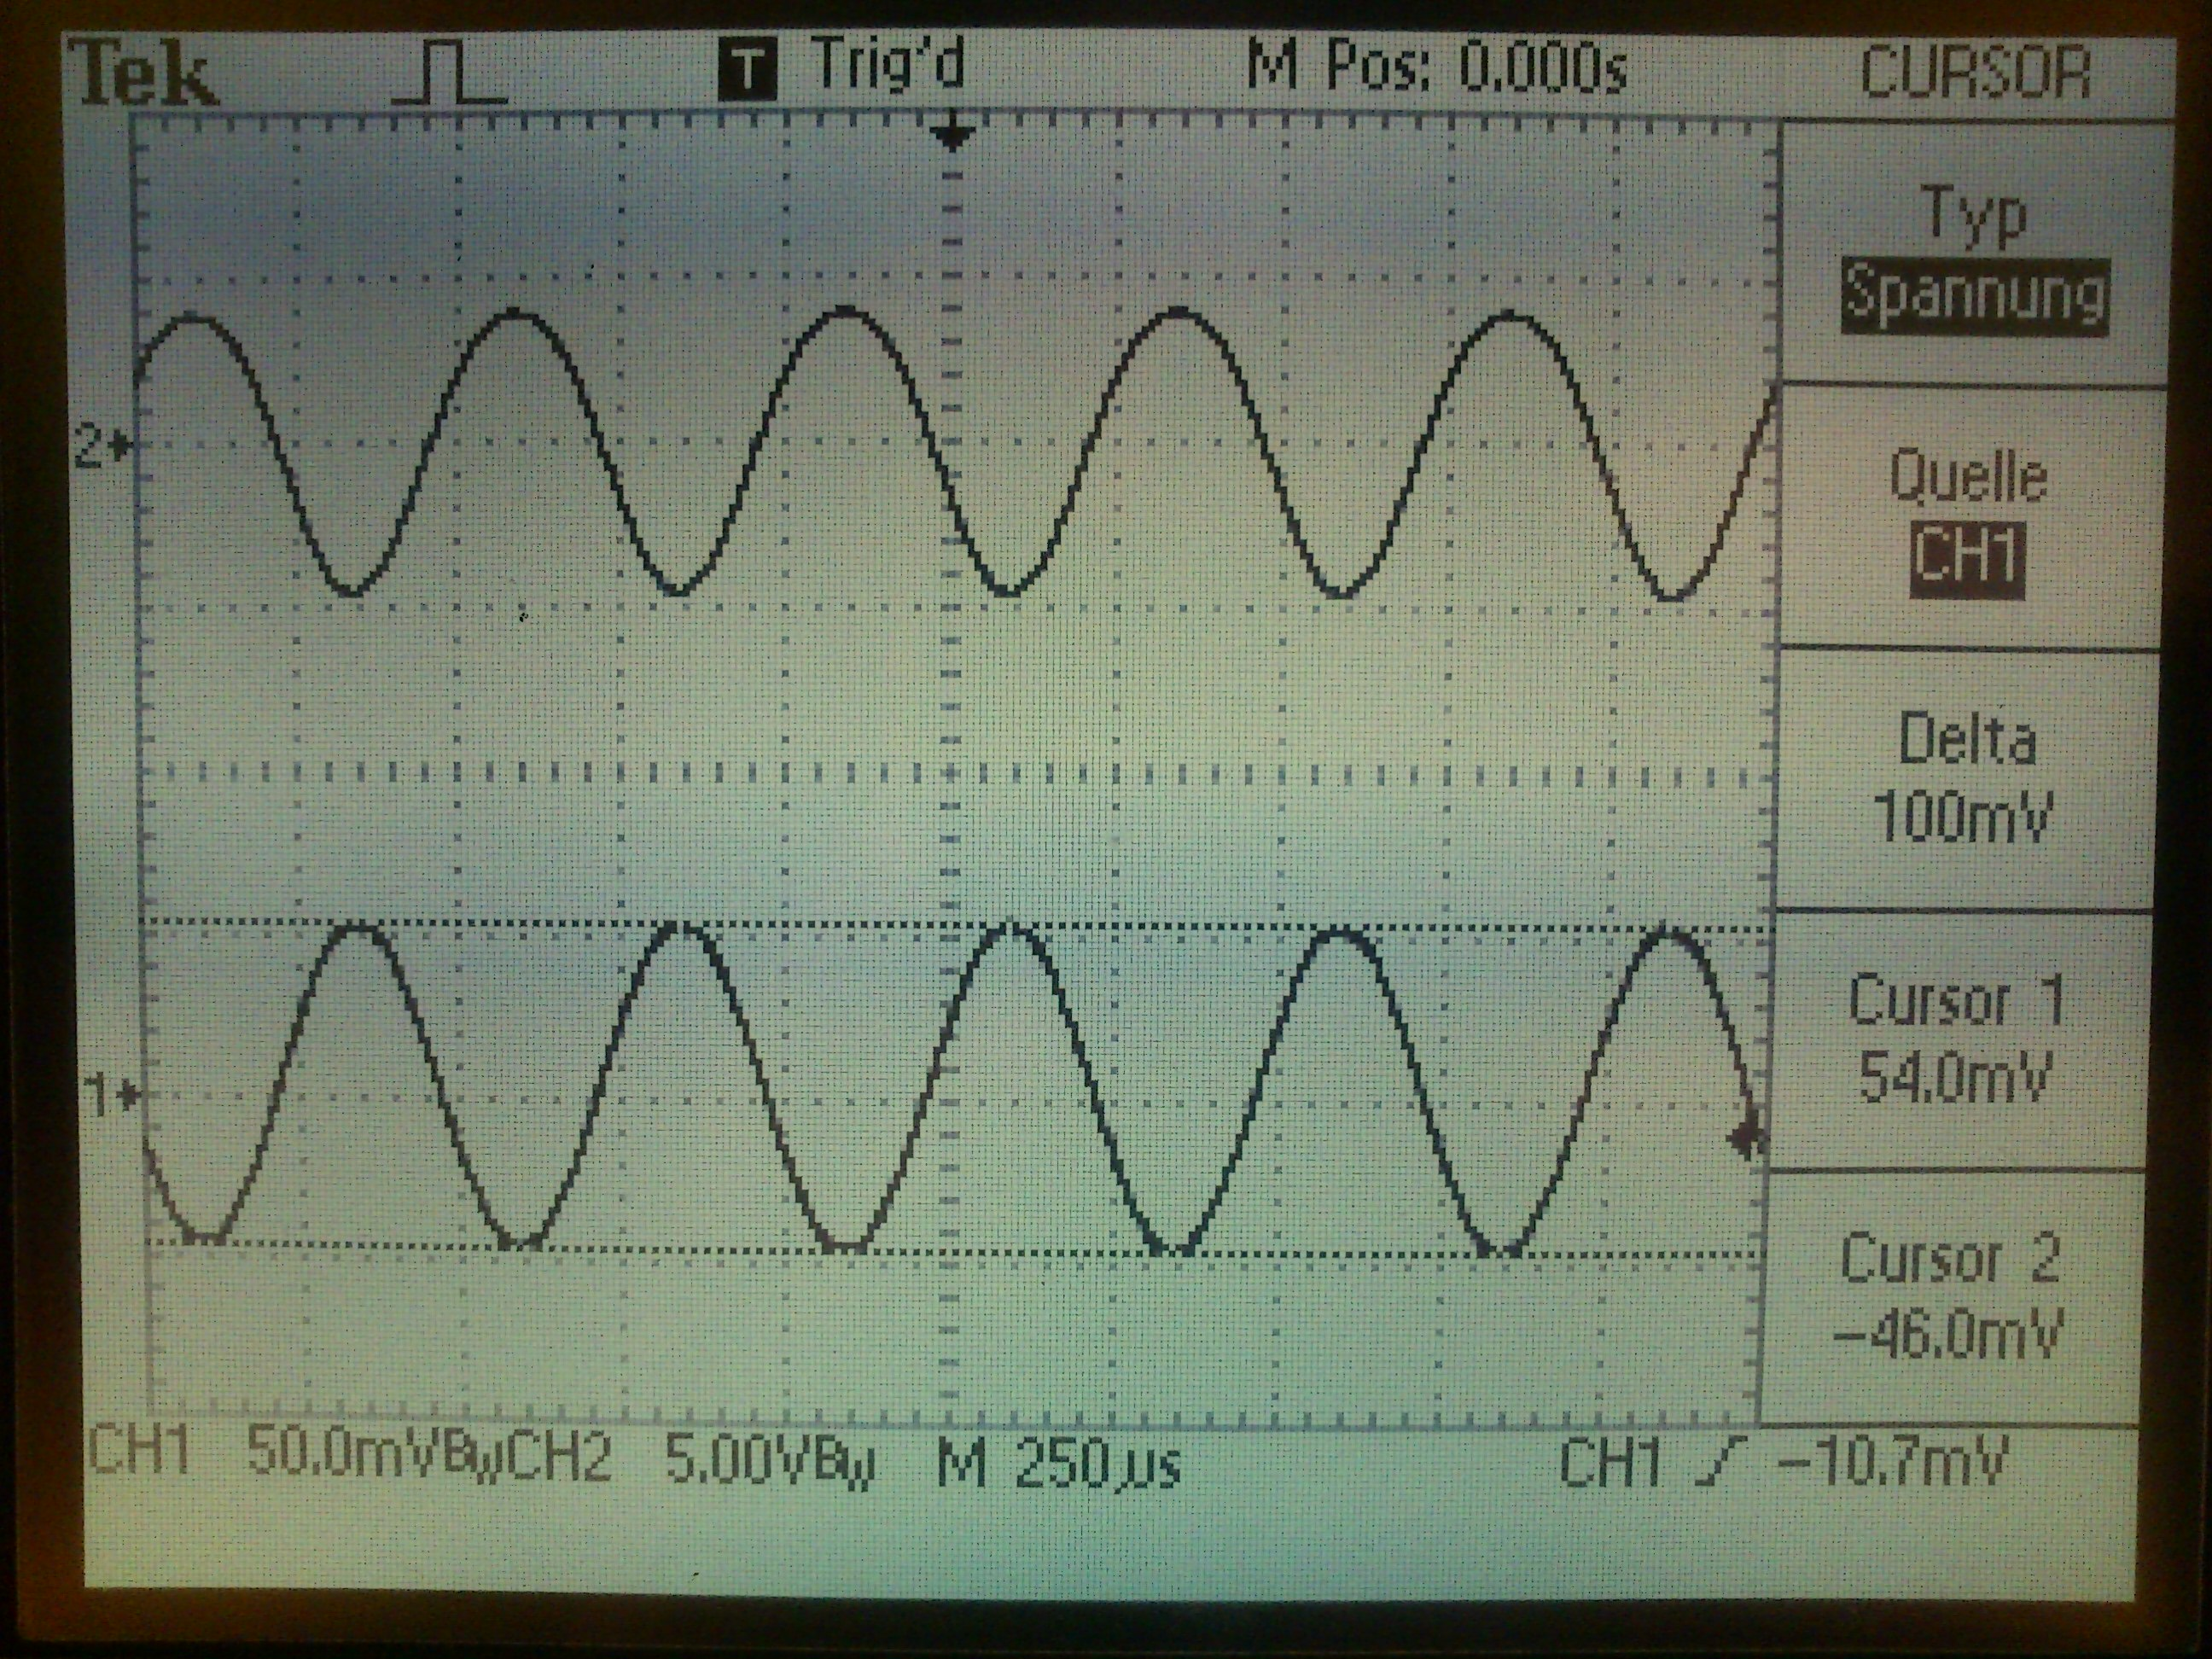
\includegraphics[width=\linewidth]{versuch5/oszi/DSC_0451.JPG}
%%%	\caption{Bestimmung der Eingangsspannung zu 100mV}
%%%\end{figure}
%%%\begin{figure}[H]
%%%	\centering
%%%	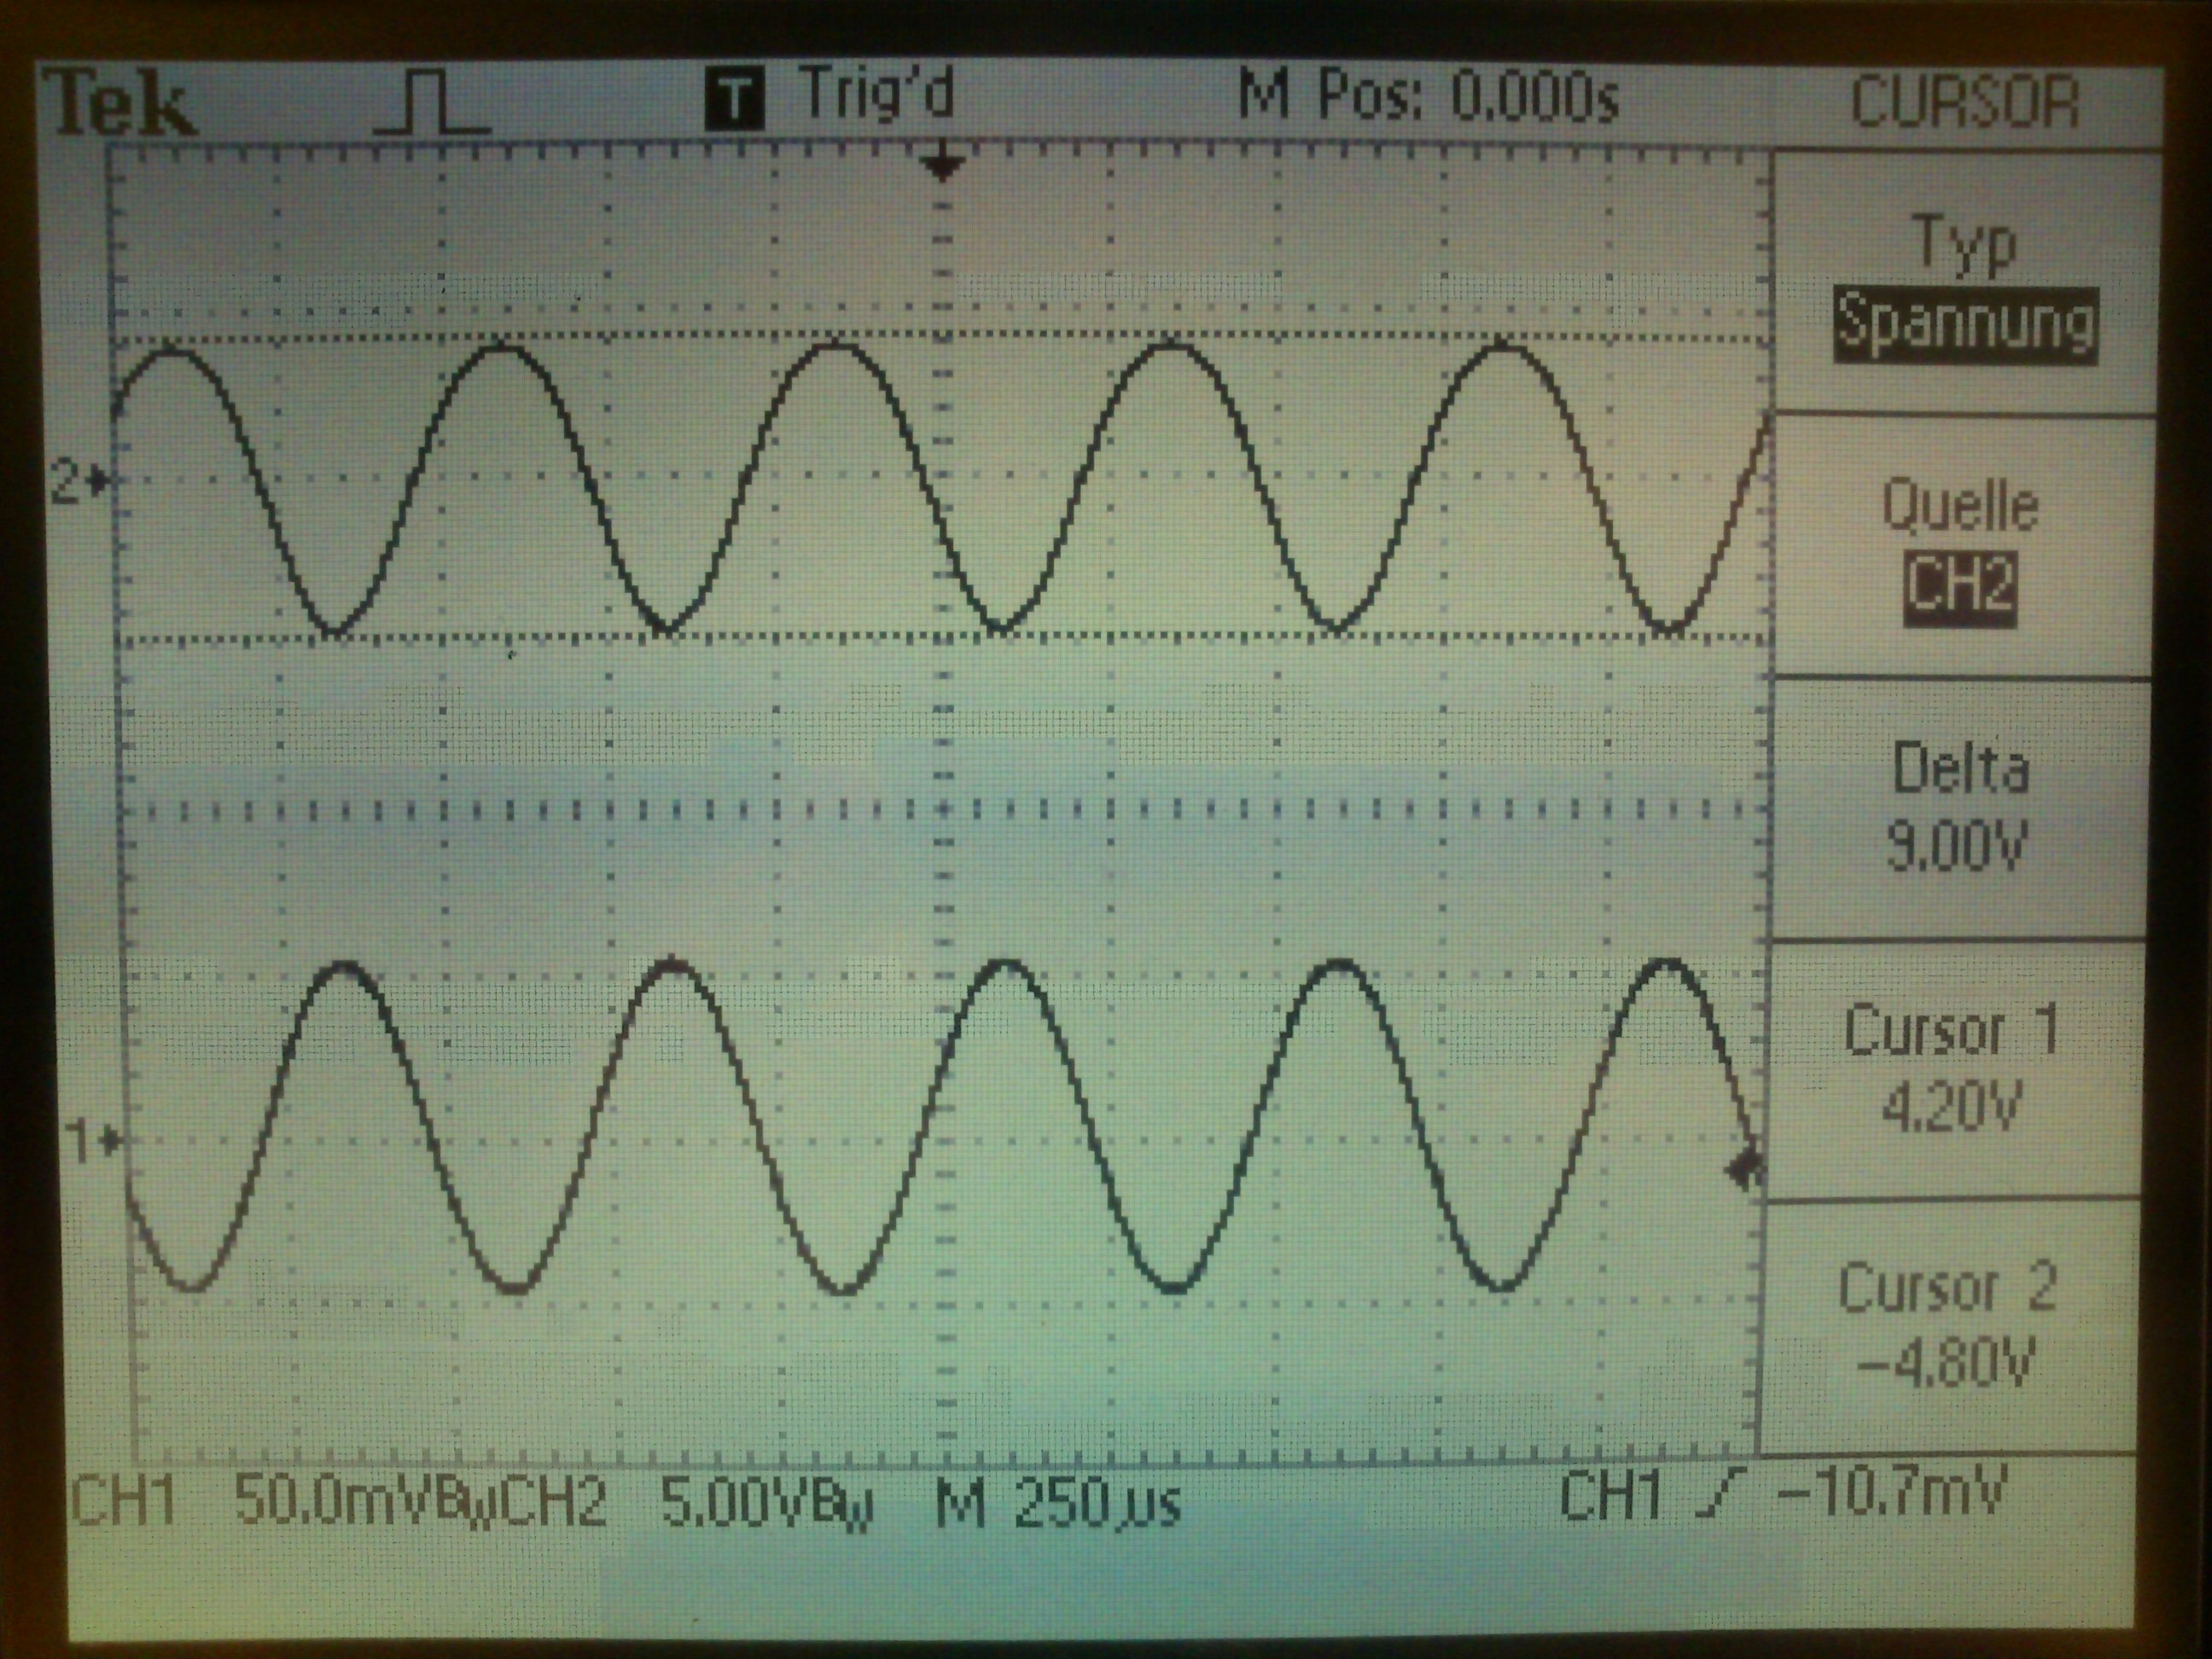
\includegraphics[width=\linewidth]{versuch5/oszi/DSC_0453.JPG}
%%%	\caption{Bestimmung der Ausgangsspannung zu 9V}
%%%\end{figure}
%%%Daraus ergibt sich die Verstärkung zu $\frac{9V}{100mV}=90$ und bleibt damit weit hinter der Erwartung zurück. Die Grenzfrequenz des Verstärkers wurde zu 370kHz bestimmt.
%%%\begin{figure}[H]
%%%	\centering
%%%	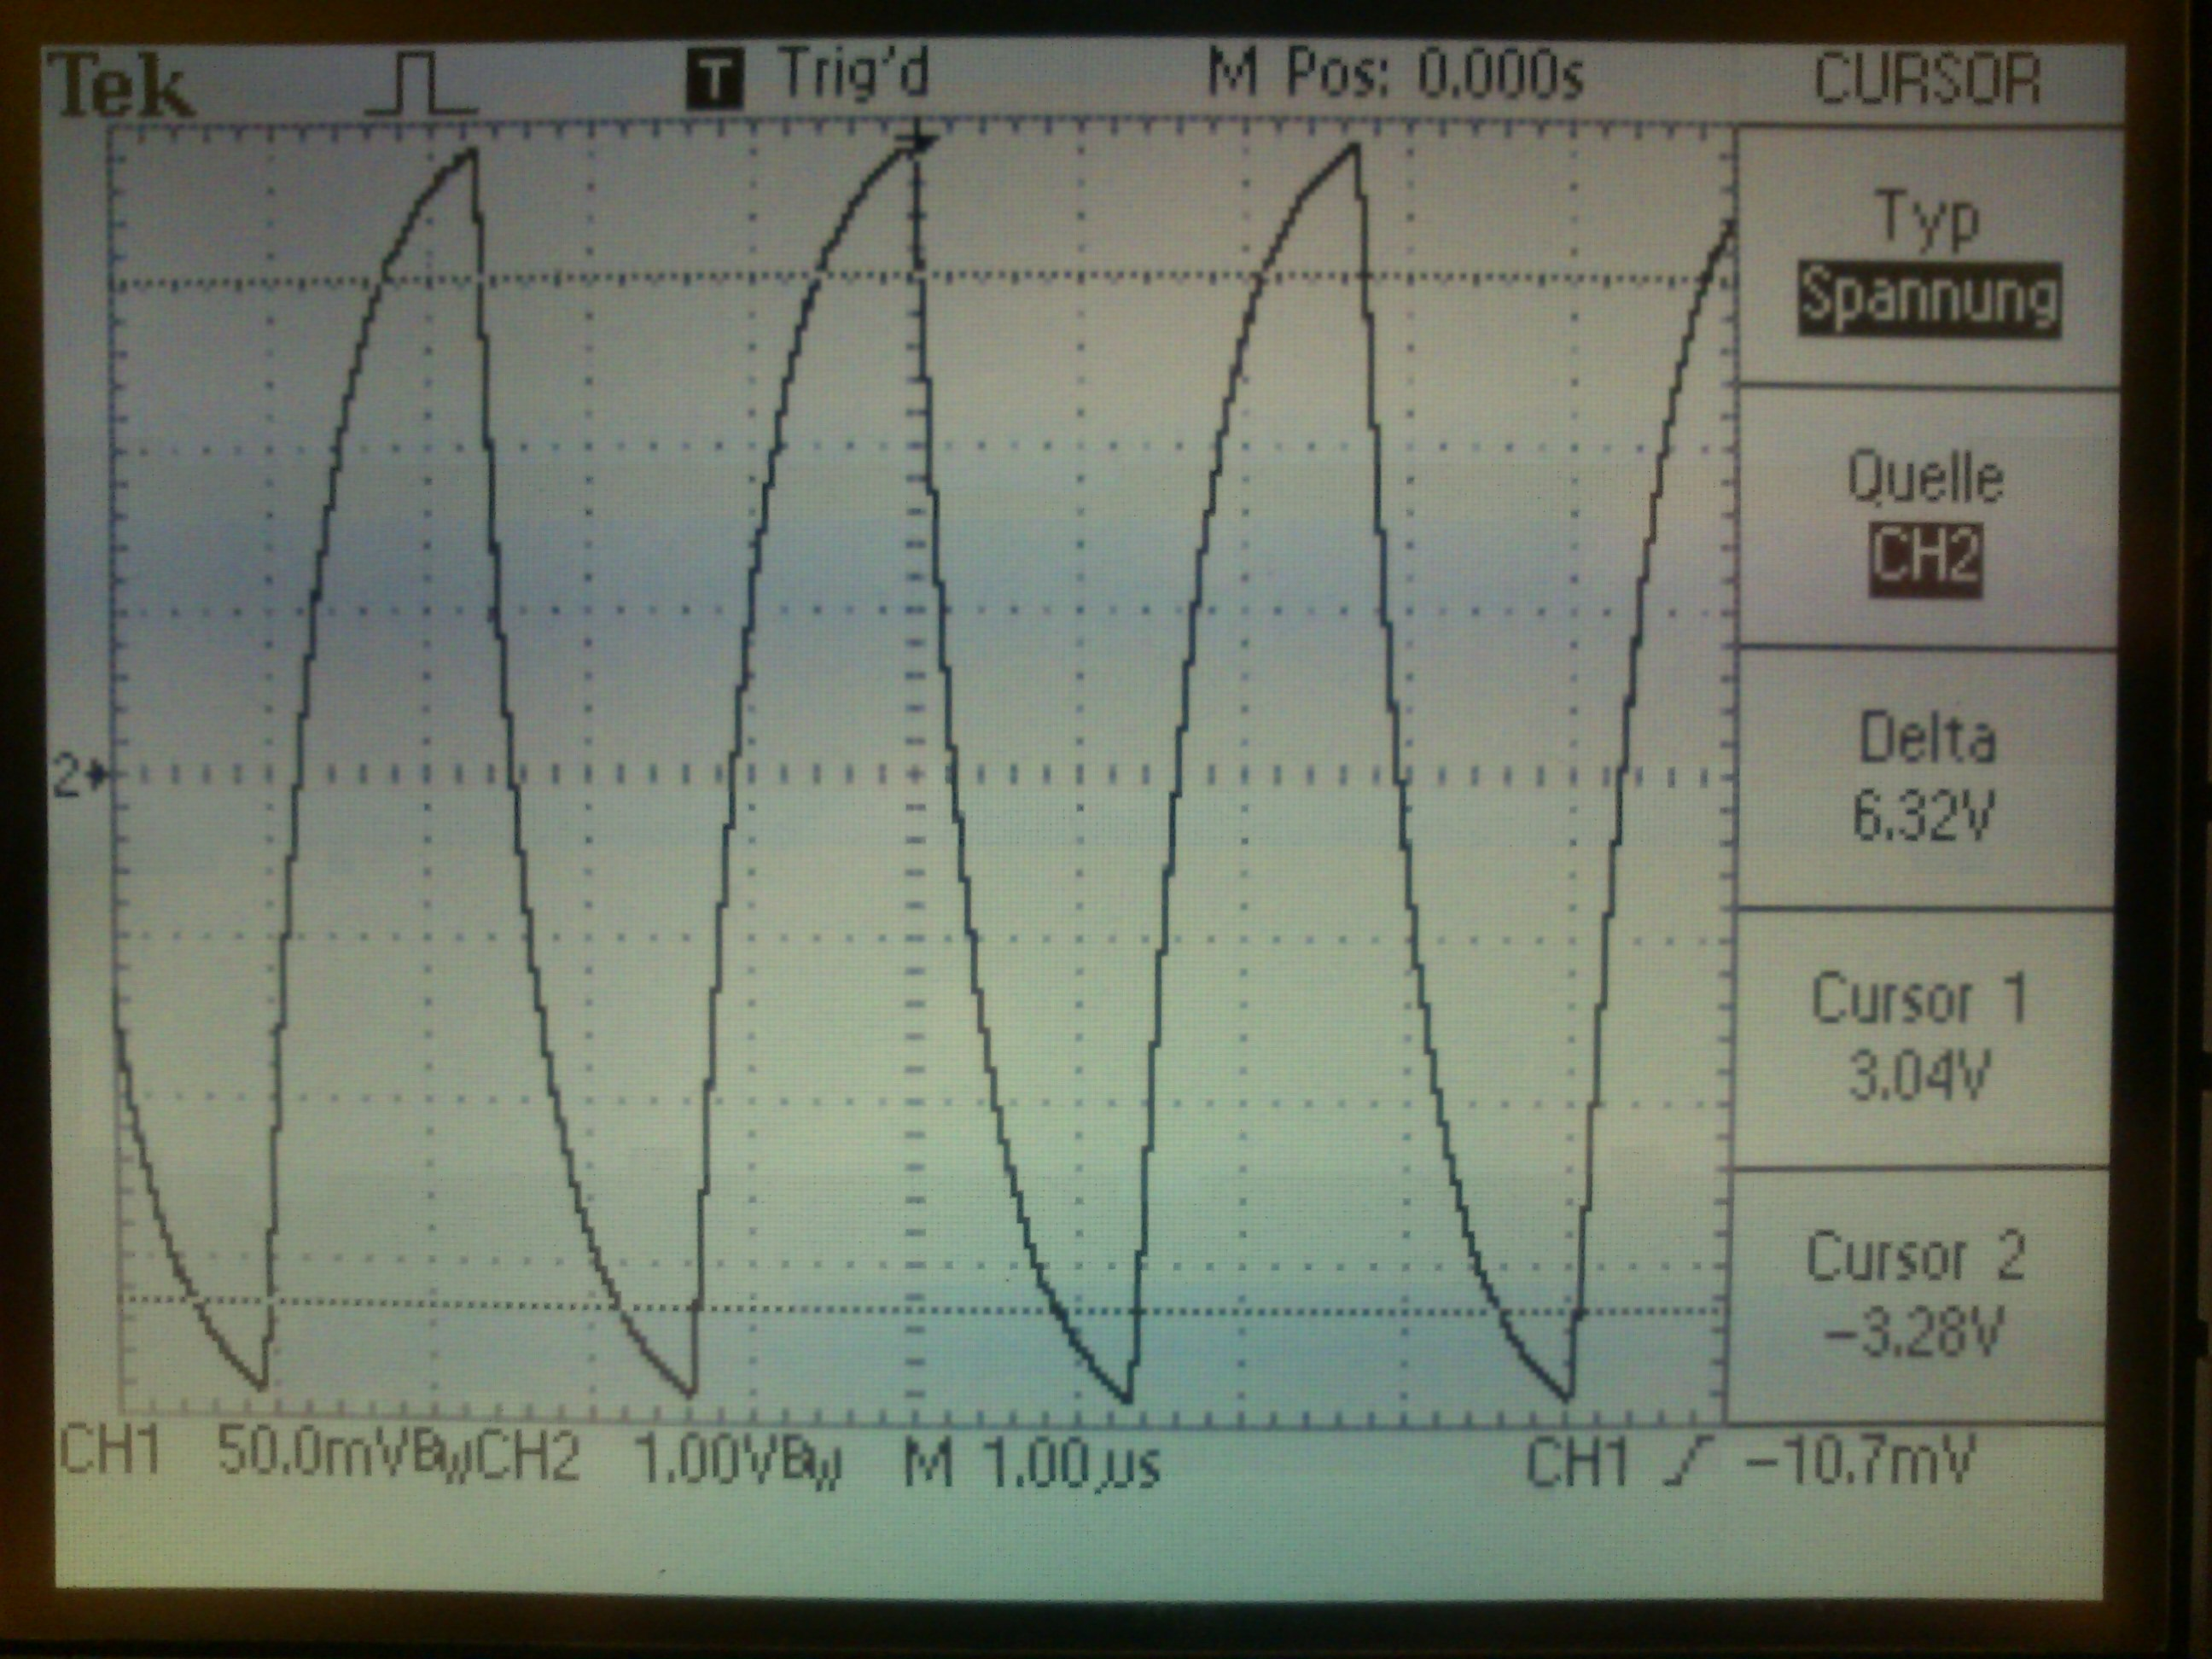
\includegraphics[width=\linewidth]{versuch5/oszi/DSC_0458.JPG}
%%%	\caption{Signalform bei Rechteckspannung}
%%%\end{figure}
%%%Die Form kommt von der Hochpasscharakteristik des Eingangsfilters her. Die steilen Signalflanken können es quasi ungedämpft passieren, wärend die normalen Signale abgeschwächt werden.
%%%
%%%Als nächstes wurde der Verstärker mit dem Digitalmultimeter verbunden und mit Kältespray behandelt. Die Spannungsverstärkung stieg dadurch an. Man sieht den Effekt nur 10 fach verstärkt, weil die Beschaltung den Transistor 'zähmt'. Durch die gesteigerte Amplitude verschiebt sich der Bezugspunkt stärker während jeder Schwingung und dämpft somit das Signal.
%%%
%%%\subsection{Transistor als Schalter}
%%%\begin{figure}[H]
%%%	\centering
%%%	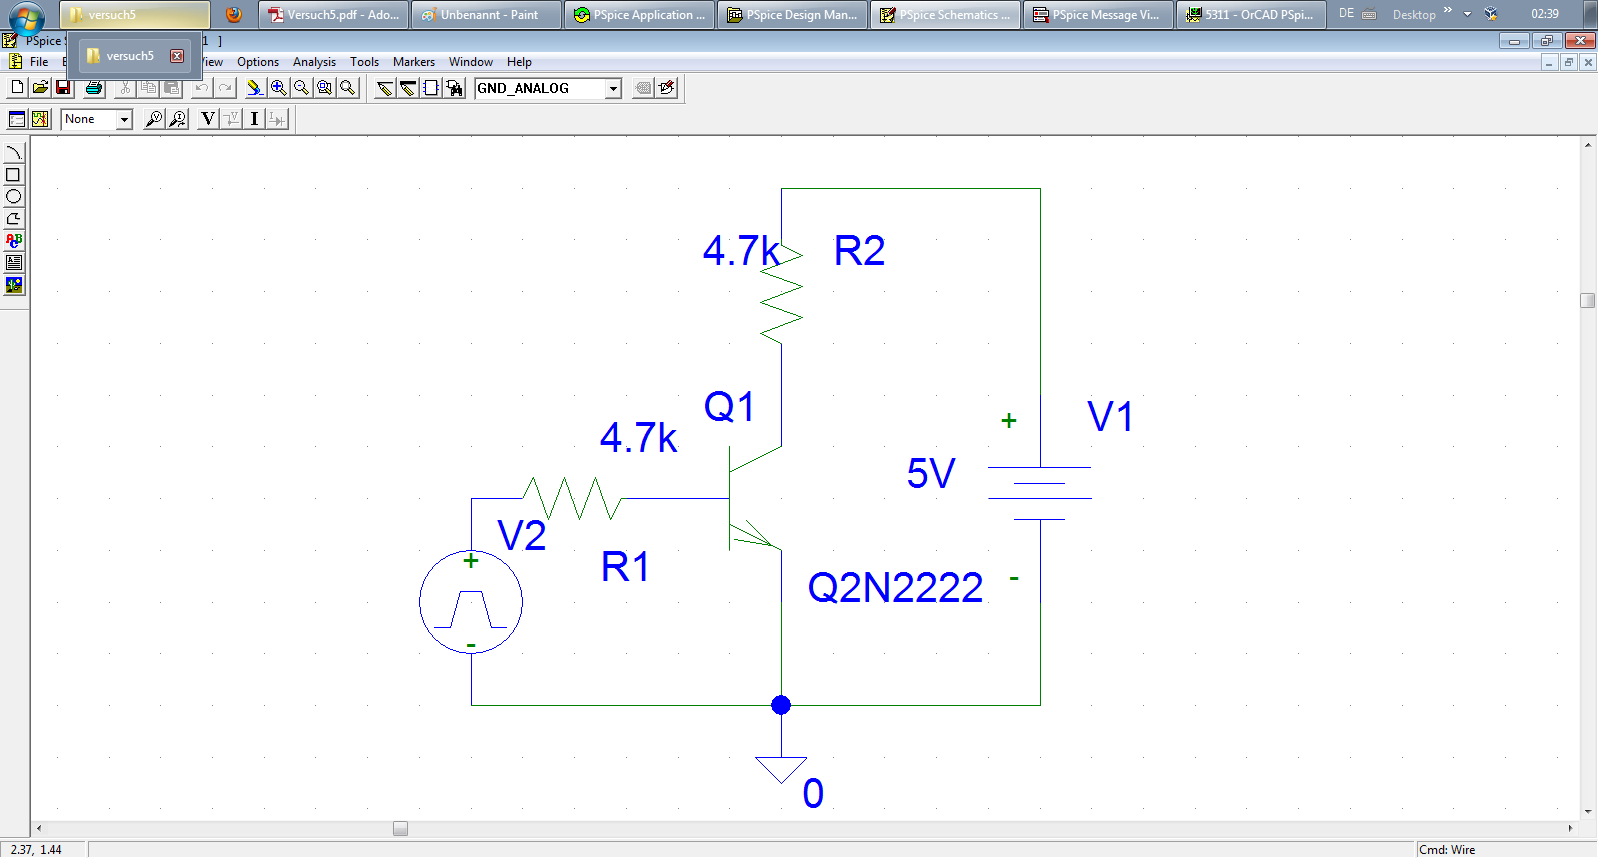
\includegraphics[width=\linewidth]{versuch5/spice/s5411.png}
%%%	\caption{Schaltplan, wie im Skript vorgegeben}
%%%\end{figure}
%%%\begin{figure}[H]
%%%	\centering
%%%	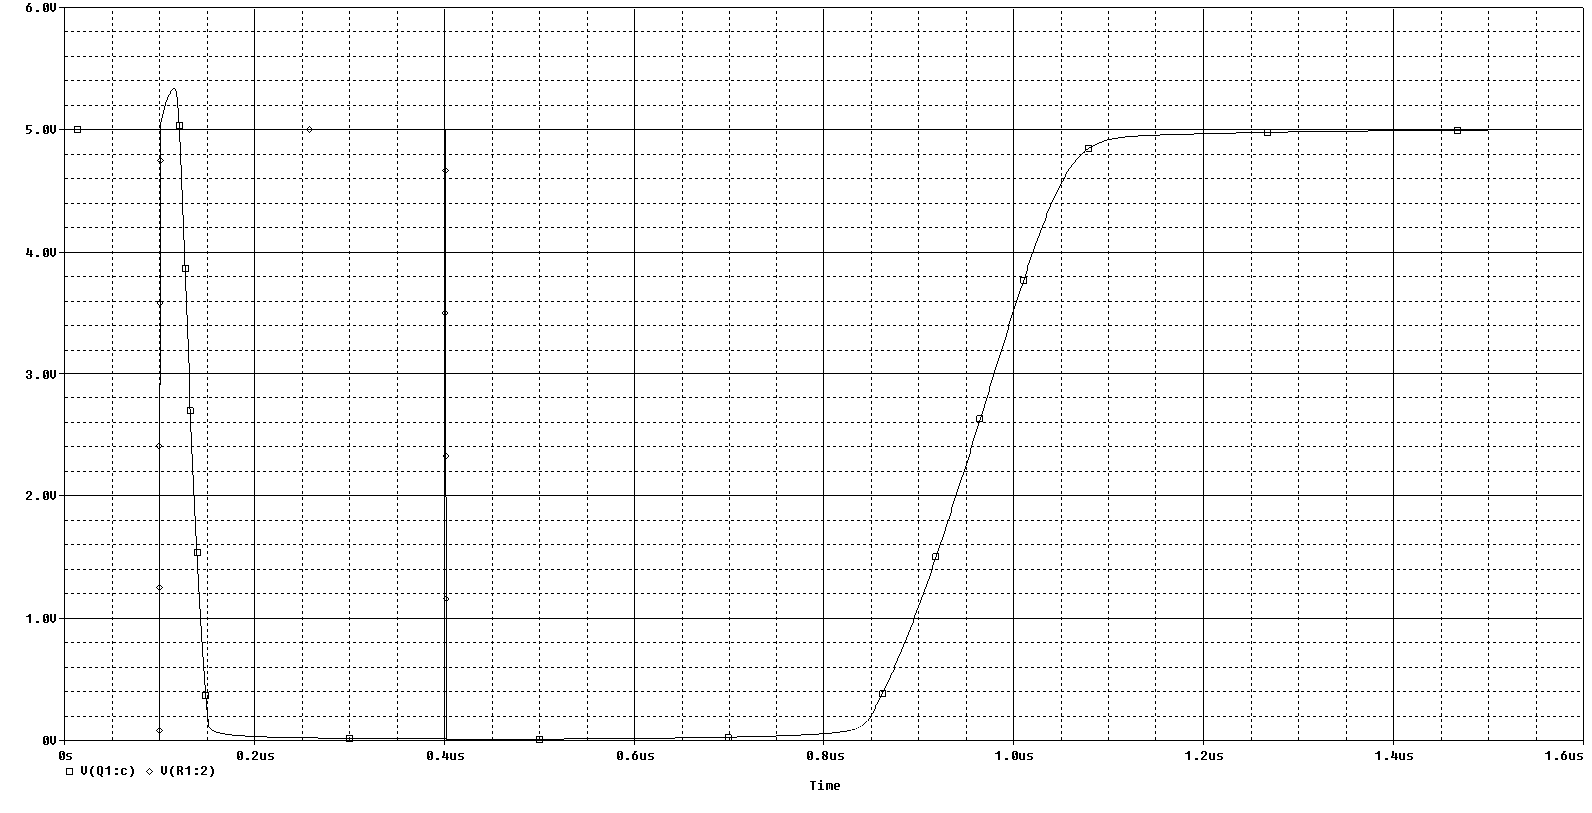
\includegraphics[width=\linewidth]{versuch5/spice/5411.png}
%%%	\caption{Simulationsergebnis}
%%%\end{figure}
%%%Die Verzögerungszeit beim Einschalten des Transistors beträgt 70ns, die Verzögerung beim Ausschalten beträgt 1100ns. Der Transistor wird in Sättigung betrieben. Bis er umschalten kann, müssen erst überschüssige Ladungen aus ihm abfließen. Wenn man eine Diode einfügt, ergibt sich folgendes:
%%%\subsubsection*{Simulation}
%%%\begin{figure}[H]
%%%	\centering
%%%	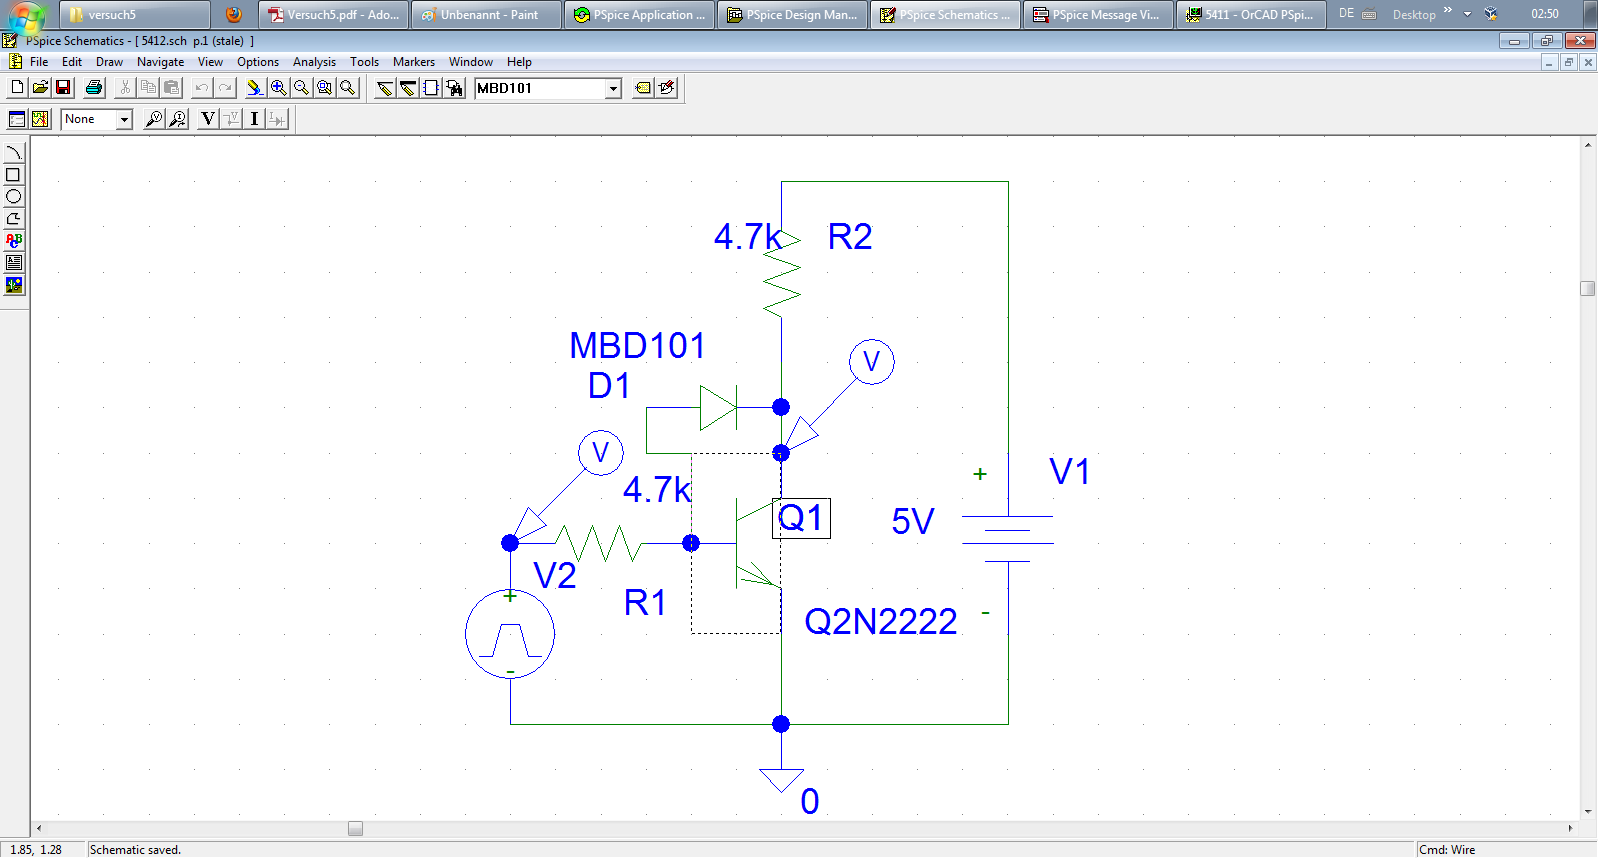
\includegraphics[width=\linewidth]{versuch5/spice/s5412.png}
%%%	\caption{Schaltplan, wie im Skript vorgegeben}
%%%\end{figure}
%%%\begin{figure}[H]
%%%	\centering
%%%	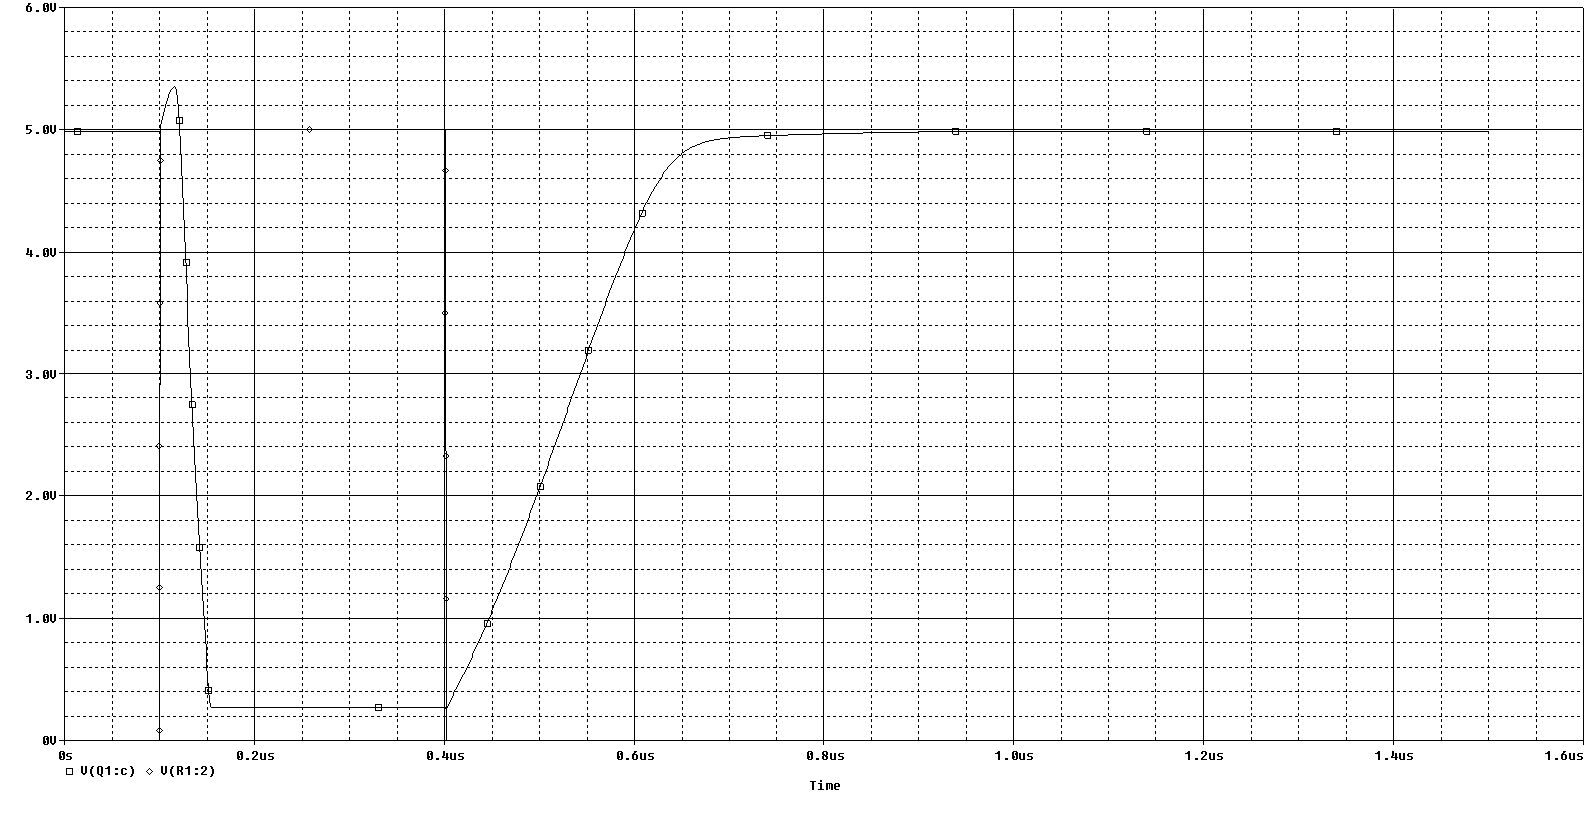
\includegraphics[width=\linewidth]{versuch5/spice/5412.png}
%%%	\caption{Simulationsergebnis}
%%%\end{figure}
%%%Durch die Diode wird das Ausschalten deutlich beschleunigt, allerdings erreicht der Schalter jetzt nicht mehr die 0V, sondern nur noch 1.1V. Die Verwendung einer PN-Diode wäre hier fatal, da sie während ihrer Speicherzeit die Versorgungsspannung niederohmig mit dem Eingangssignal verbände.
%%%
%%%\subsection{Transistor als Schalter mit induktiver Last}
%%%\begin{figure}[H]
%%%	\centering
%%%	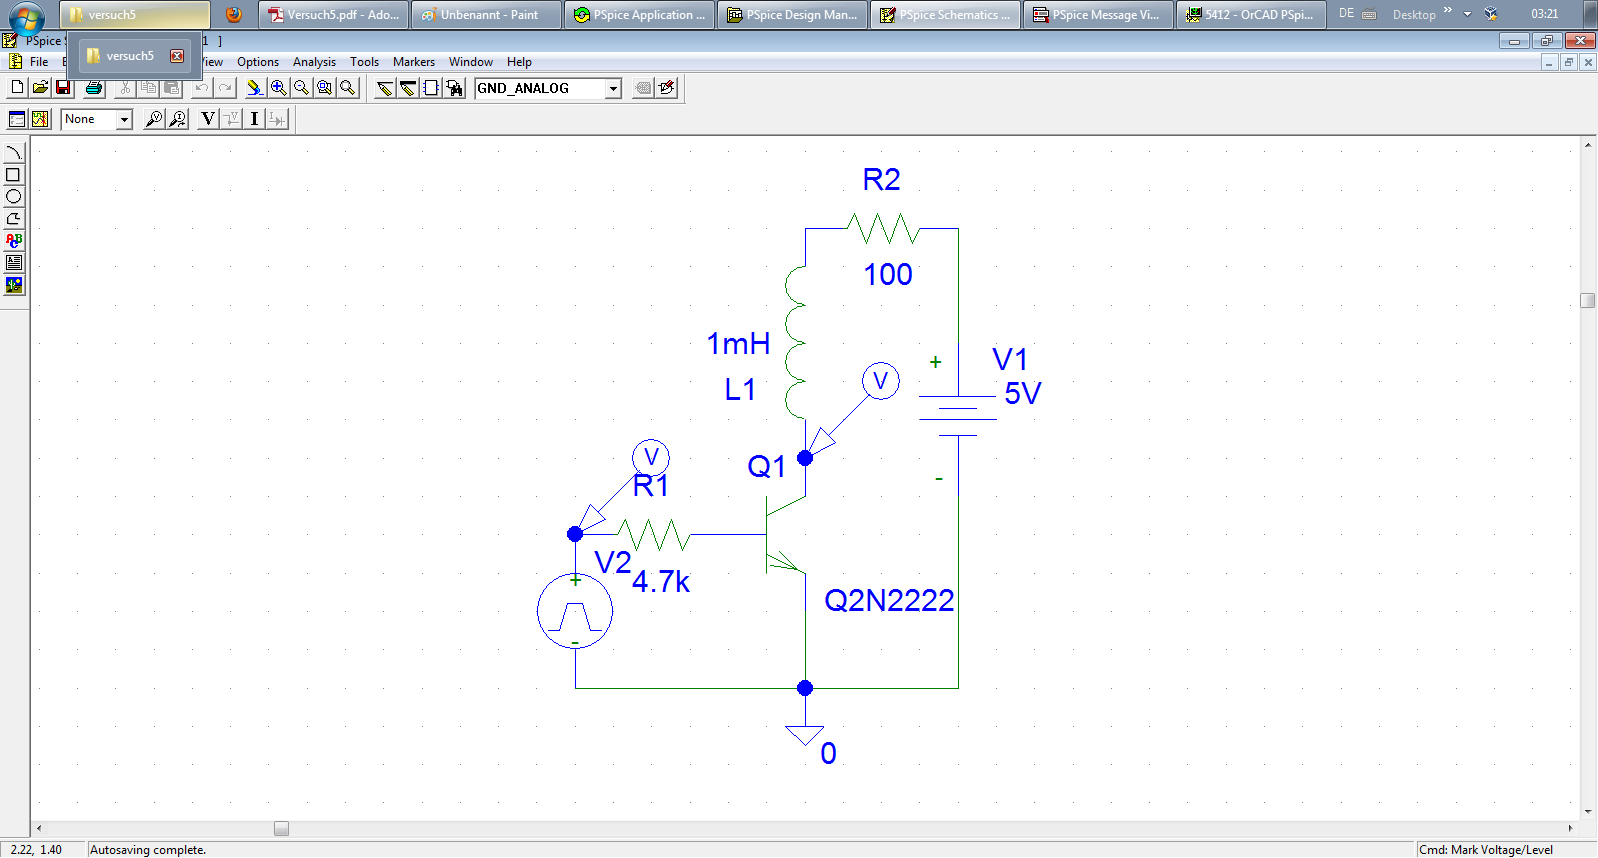
\includegraphics[width=\linewidth]{versuch5/spice/s5511.png}
%%%	\caption{Schaltplan, wie im Skript vorgegeben}
%%%\end{figure}
%%%\begin{figure}[H]
%%%	\centering
%%%	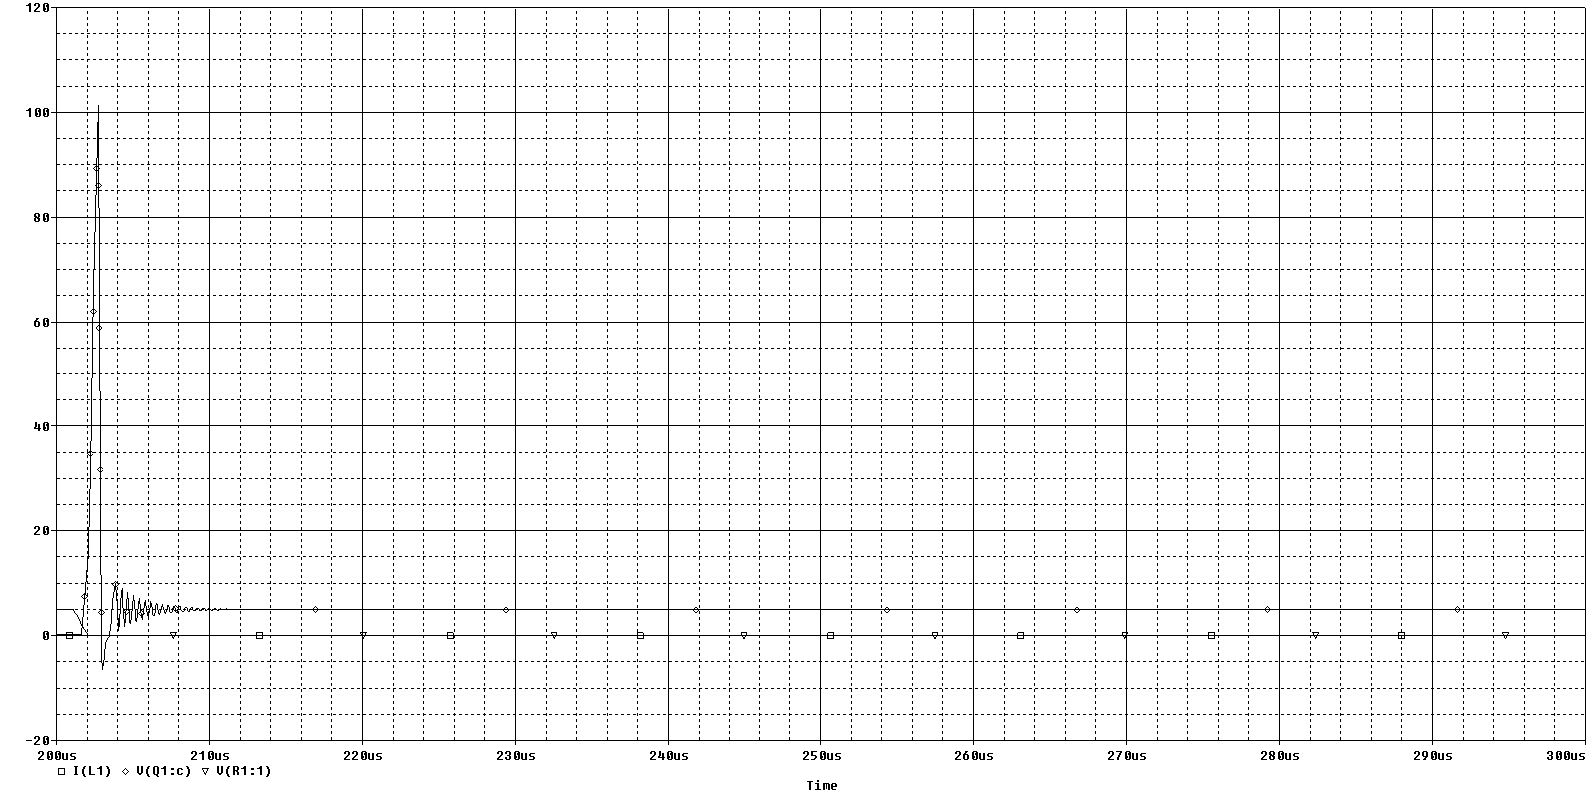
\includegraphics[width=\linewidth]{versuch5/spice/5511.png}
%%%	\caption{Simulationsergebnis}
%%%\end{figure}
%%%\begin{figure}[H]
%%%	\centering
%%%	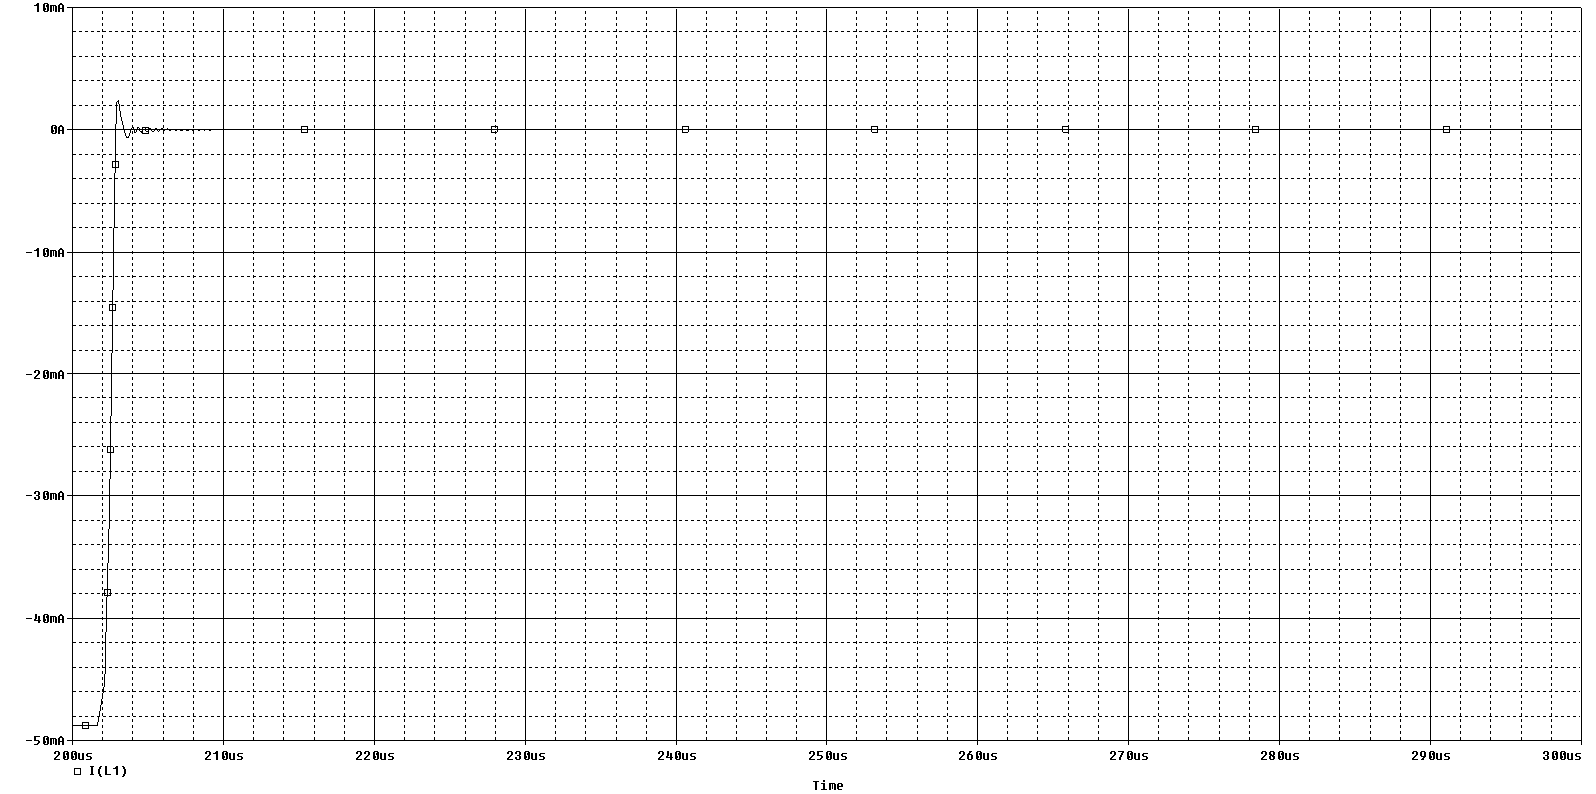
\includegraphics[width=\linewidth]{versuch5/spice/5511I.png}
%%%	\caption{Simulationsergebnis: Strom}
%%%\end{figure}
%%%Der Transistor wird nicht lange überleben, weil er plötzlich gut 105V ableiten muss, wofür er sehr wahrscheinlich nicht gemacht war.\\ Die maximale Stromänderung wurde mit folgenden beiden Wertepaaren bestimmt (202.252\µs, -40.996mA) und (202.782\µs, -5.7515mA):
%%%\[ \Delta I_{max}=\frac{-40.996+5.7515}{202.252-202.782}=-0.1819 \frac{A}{\µs}\]
%%%Damit ergibt sich die Induzierte Spannung zu
%%%\[ U_{IND} = -L*\frac{\Delta I}{\Delta t};\; L=1mH,\; \frac{\Delta I}{\Delta t}=-0.1819 \frac{A}{\µs} \]
%%%\[ \Rightarrow \; U_{IND}=\frac{1mH*0.1819A}{1\µs}=\frac{0.1819HA}{1ms}=\frac{181.9HA}{1s}=181.9V \]
%%%\begin{figure}[H]
%%%	\centering
%%%	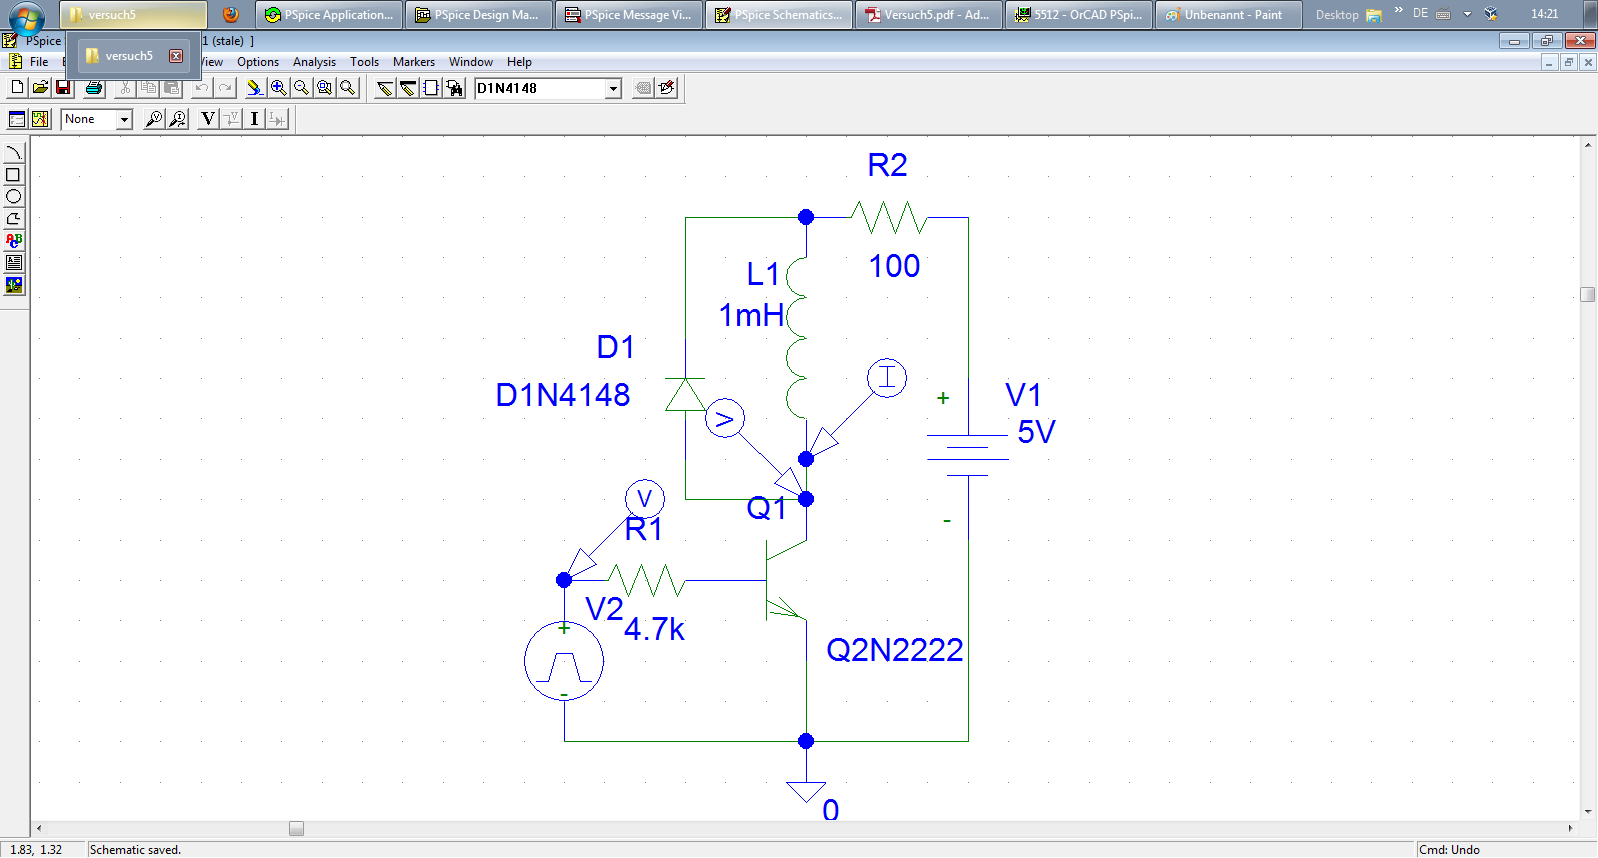
\includegraphics[width=\linewidth]{versuch5/spice/s5512.png}
%%%	\caption{Schaltplan, mit Diode}
%%%\end{figure}
%%%\begin{figure}[H]
%%%	\centering
%%%	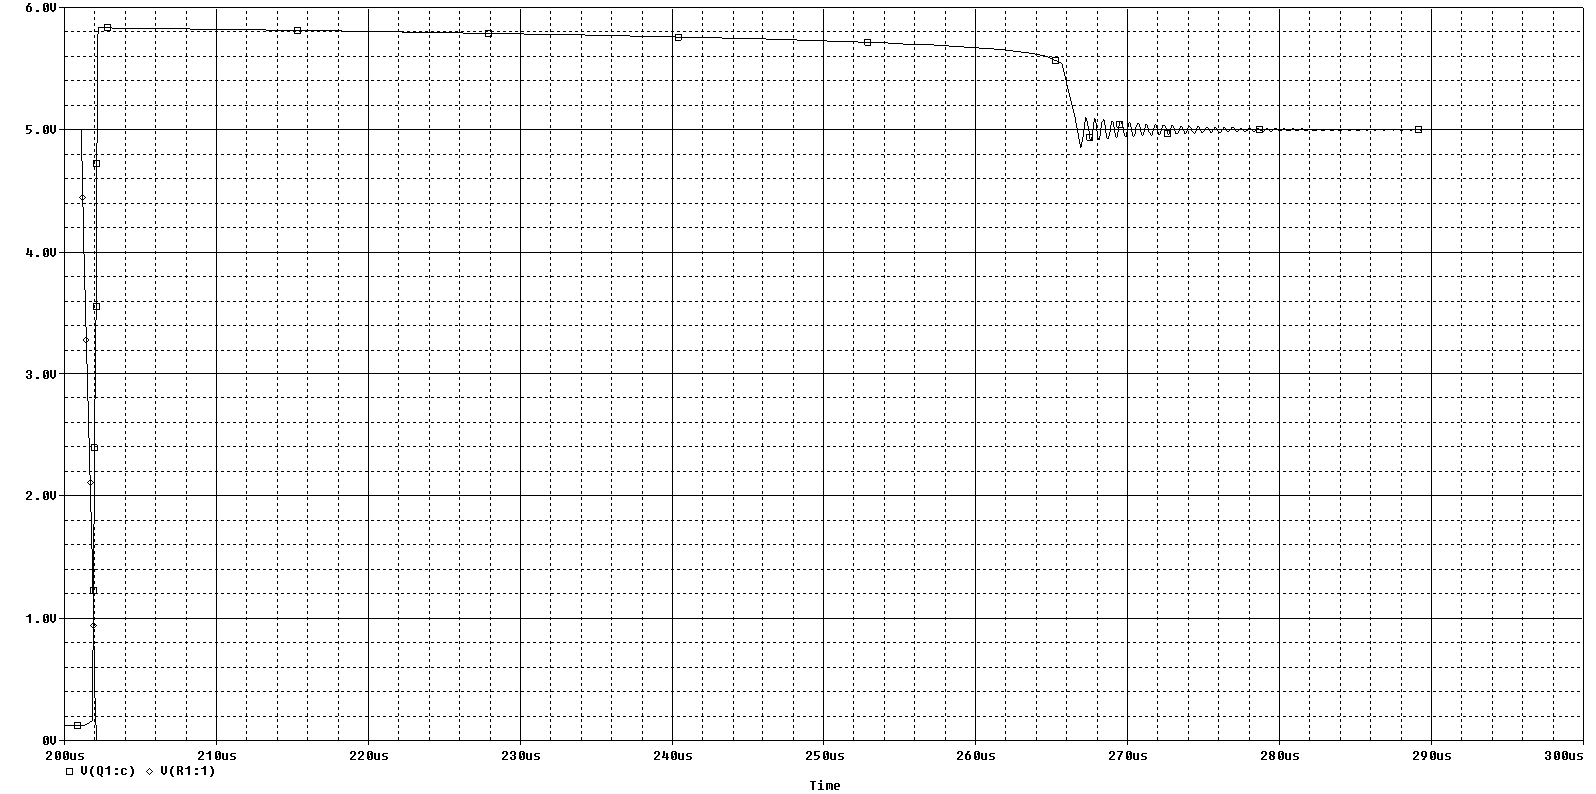
\includegraphics[width=\linewidth]{versuch5/spice/5512.png}
%%%	\caption{Simulationsergebnis: Die Spannungsspitze wird durch die Diode abgeleitet}
%%%\end{figure}
%%%\begin{figure}[H]
%%%	\centering
%%%	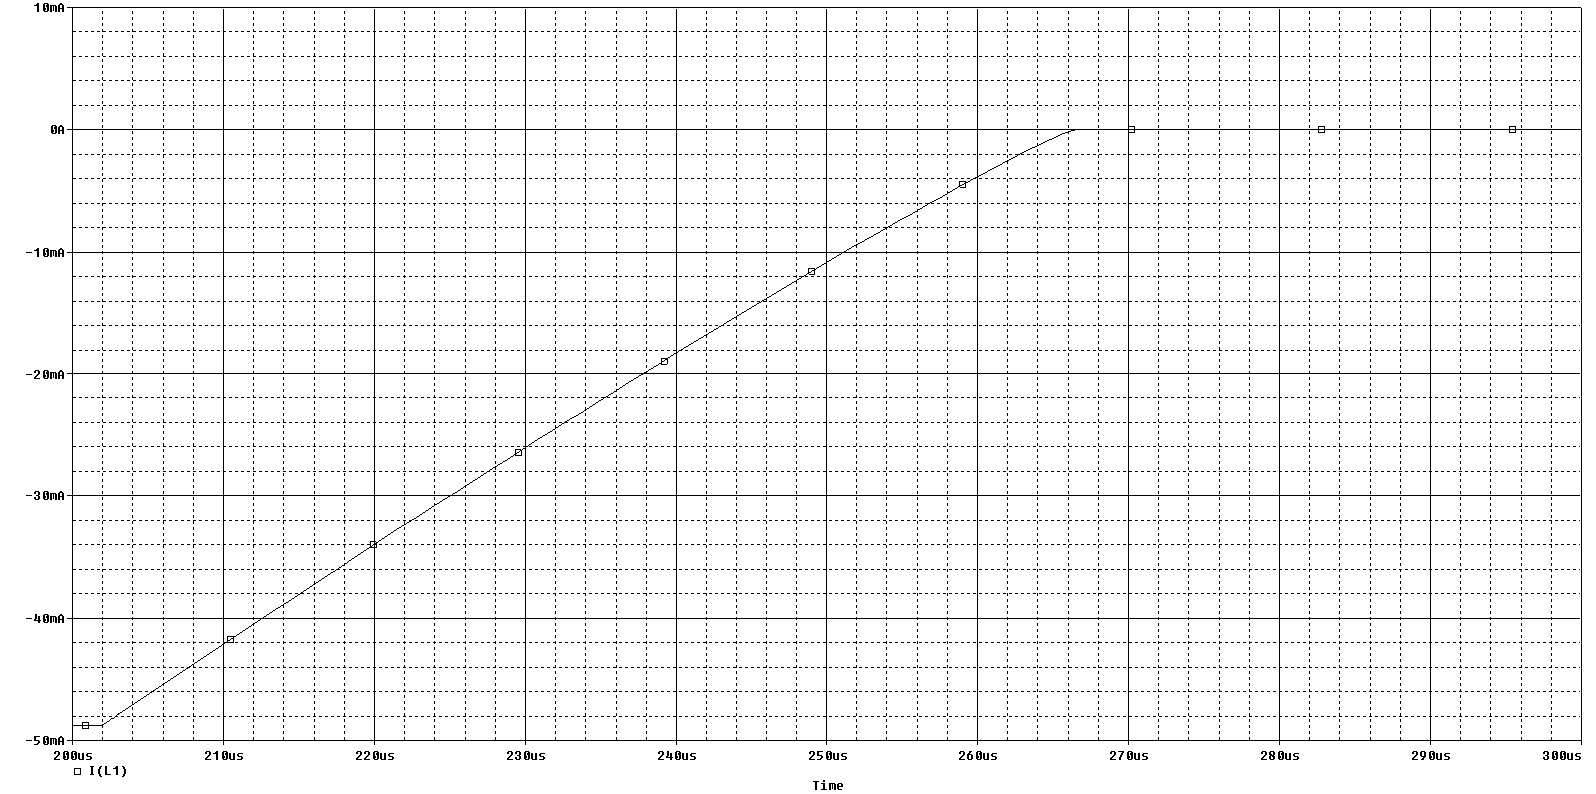
\includegraphics[width=\linewidth]{versuch5/spice/5512I.png}
%%%	\caption{Simulationsergebnis: \Delta I deutlich geringer}
%%%\end{figure}
%%%
%%%
%%%
%%%
%%%
%%%
%%%
%%%
%%%
%%%
%%%
%%%
%%%
%%%
%%%
%%%
%%%
%%%
%%%
%%%
%%%
%%%
%%%
%%%
%%%
%%%
%%%
%%%
%%%
%%%
%%%
%%%
%%%
%%%%}}}
%%%
%%%
%%%



